\documentclass[11pt]{charter}
%DIF LATEXDIFF DIFFERENCE FILE
%DIF DEL Past.tex      Sun Aug  9 19:27:56 2020
%DIF ADD charter.tex   Sun Aug  9 19:28:12 2020
% !TeX spellcheck = es
% El títulos de la memoria, se usa en la carátula y se puede usar el cualquier lugar del documento con el comando \ttitle
\titulo{Sistema de actualización remota de firmware a través de una red LoRaWAN} 

% Nombre del posgrado, se usa en la carátula y se puede usar el cualquier lugar del documento con el comando \degreename
\posgrado{Carrera de Especialización en Sistemas Embebidos} 
%\posgrado{Carrera de Especialización en Internet de las Cosas} 
%\posgrado{Carrera de Especialización en Intelegencia Artificial}
%\posgrado{Maestría en Sistemas Embebidos} 
%\posgrado{Maestría en Internet de las cosas}

% Tu nombre, se puede usar el cualquier lugar del documento con el comando \authorname
\autor{Ronal Celaya} 

% El nombre del director y co-director, se puede usar el cualquier lugar del documento con el comando \supname y \cosupname y \pertesupname y \pertecosupname
%DIF 17-18c17-18
%DIF < \director{Nombre del Director}
%DIF < \pertenenciaDirector{pertenencia} 
%DIF -------
\director{Osvaldo Ivani} %DIF > 
\pertenenciaDirector{SMARTIUM, S. A.}  %DIF > 
%DIF -------
% FIXME:NO IMPLEMENTADO EL CODIRECTOR ni su pertenencia
%DIF 20-21c20-21
%DIF < \codirector{} % si queda vacio no se deberíá incluir 
%DIF < \pertenenciaCoDirector{}
%DIF -------
\codirector{Jhonattan Camargo} % si queda vacio no se deberíá incluir  %DIF > 
\pertenenciaCoDirector{SMARTIUM, S. A.} %DIF > 
%DIF -------

% Nombre del cliente, quien va a aprobar los resultados del proyecto, se puede usar con el comando \clientename y \empclientename
\cliente{Osvaldo Ivani}
\empresaCliente{SMARTIUM, S. A.}

% Nombre y pertenencia de los jurados, se pueden usar el cualquier lugar del documento con el comando \jurunoname, \jurdosname y \jurtresname y \perteunoname, \pertedosname y \pertetresname.
\juradoUno{Nombre y Apellido (1)}
\pertenenciaJurUno{pertenencia (1)} 
\juradoDos{Nombre y Apellido (2)}
\pertenenciaJurDos{pertenencia (2)}
\juradoTres{Nombre y Apellido (3)}
\pertenenciaJurTres{pertenencia (3)}
 
\fechaINICIO{27 de junio de 2020}		%Fecha de inicio de la cursada de GdP \fechaInicioName
\fechaFINALPlanificacion{22 de Agosto de 2020} 	%Fecha de final de cursada de GdP
%DIF < \fechaFINALTrabajo{22 de diciembre de 2020}		%Fecha de defensa pública del trabajo final
%DIF -------
\fechaFINALTrabajo{01 de Abril de 2021}		%Fecha de defensa pública del trabajo final %DIF > 
%DIF PREAMBLE EXTENSION ADDED BY LATEXDIFF
%DIF UNDERLINE PREAMBLE %DIF PREAMBLE
\RequirePackage[normalem]{ulem} %DIF PREAMBLE
\RequirePackage{color}\definecolor{RED}{rgb}{1,0,0}\definecolor{BLUE}{rgb}{0,0,1} %DIF PREAMBLE
\providecommand{\DIFadd}[1]{{\protect\color{blue}\uwave{#1}}} %DIF PREAMBLE
\providecommand{\DIFdel}[1]{{\protect\color{red}\sout{#1}}}                      %DIF PREAMBLE
%DIF SAFE PREAMBLE %DIF PREAMBLE
\providecommand{\DIFaddbegin}{} %DIF PREAMBLE
\providecommand{\DIFaddend}{} %DIF PREAMBLE
\providecommand{\DIFdelbegin}{} %DIF PREAMBLE
\providecommand{\DIFdelend}{} %DIF PREAMBLE
\providecommand{\DIFmodbegin}{} %DIF PREAMBLE
\providecommand{\DIFmodend}{} %DIF PREAMBLE
%DIF FLOATSAFE PREAMBLE %DIF PREAMBLE
\providecommand{\DIFaddFL}[1]{\DIFadd{#1}} %DIF PREAMBLE
\providecommand{\DIFdelFL}[1]{\DIFdel{#1}} %DIF PREAMBLE
\providecommand{\DIFaddbeginFL}{} %DIF PREAMBLE
\providecommand{\DIFaddendFL}{} %DIF PREAMBLE
\providecommand{\DIFdelbeginFL}{} %DIF PREAMBLE
\providecommand{\DIFdelendFL}{} %DIF PREAMBLE
%DIF LISTINGS PREAMBLE %DIF PREAMBLE
\RequirePackage{listings} %DIF PREAMBLE
\RequirePackage{color} %DIF PREAMBLE
\lstdefinelanguage{DIFcode}{ %DIF PREAMBLE
%DIF DIFCODE_UNDERLINE %DIF PREAMBLE
  moredelim=[il][\color{red}\sout]{\%DIF\ <\ }, %DIF PREAMBLE
  moredelim=[il][\color{blue}\uwave]{\%DIF\ >\ } %DIF PREAMBLE
} %DIF PREAMBLE
\lstdefinestyle{DIFverbatimstyle}{ %DIF PREAMBLE
	language=DIFcode, %DIF PREAMBLE
	basicstyle=\ttfamily, %DIF PREAMBLE
	columns=fullflexible, %DIF PREAMBLE
	keepspaces=true %DIF PREAMBLE
} %DIF PREAMBLE
\lstnewenvironment{DIFverbatim}{\lstset{style=DIFverbatimstyle}}{} %DIF PREAMBLE
\lstnewenvironment{DIFverbatim*}{\lstset{style=DIFverbatimstyle,showspaces=true}}{} %DIF PREAMBLE
%DIF END PREAMBLE EXTENSION ADDED BY LATEXDIFF

\begin{document}

\maketitle
\thispagestyle{empty}
\pagebreak


\thispagestyle{empty}
{\setlength{\parskip}{0pt}
\tableofcontents{}
}
\pagebreak


\section{Registros de cambios}
\label{sec:registro}


\begin{table}[ht]
\label{tab:registro}
\centering

\begin{tabularx}{\linewidth}{@{}|c|X|c|@{}}
\hline
\rowcolor[HTML]{C0C0C0} 
Revisión & \multicolumn{1}{c|}{\cellcolor[HTML]{C0C0C0}Detalles de los cambios realizados} & Fecha      \\ \hline
1.0      & Creación del documento                                                          & 27/06/2020 \\ \hline
1.1      & Desarrollo de las secciones 1 hasta la 6										   & 09/07/2020 \\ \hline
\end{tabularx}
\end{table}

\pagebreak



\section{Acta de \DIFdelbegin \DIFdel{Constitución }\DIFdelend \DIFaddbegin \DIFadd{constitución }\DIFaddend del \DIFdelbegin \DIFdel{Proyecto}\DIFdelend \DIFaddbegin \DIFadd{proyecto}\DIFaddend }
\label{sec:acta}

\begin{flushright}
Buenos Aires, \fechaInicioName
\end{flushright}

\vspace{2cm}

Por medio de la presente se acuerda con el Ing. \authorname\hspace{1px} que su Trabajo Final de la \degreename\hspace{1px} se titulará ``\ttitle'', consistirá esencialmente en el prototipo preliminar de un \textcolor{black}{sistema que realice la actualización remota de firmware (FUOTA, por sus siglas en inglés Firmware Update Over The Air) a través de una red LoRaWAN.}, y tendrá un presupuesto preliminar estimado de \DIFdelbegin \DIFdel{600 }\DIFdelend \DIFaddbegin \DIFadd{602 }\DIFaddend hs de trabajo, con fecha de inicio \fechaInicioName\hspace{1px} y fecha de presentación pública \fechaFinalName.

Se adjunta a esta acta la planificación inicial.

\vfill

% Esta parte se construye sola con la información que hayan cargado en el preámbulo del documento y no debe modificarla
\begin{table}[ht]
\centering
\begin{tabular}{ccc}
\begin{tabular}[c]{@{}c@{}}Ariel Lutenberg \\ Director posgrado FIUBA\end{tabular} &  & \begin{tabular}[c]{@{}c@{}}\clientename \\ \empclientename \end{tabular} \vspace{2.5cm} \\ 
\multicolumn{3}{c}{\begin{tabular}[c]{@{}c@{}} \supname \\ Director del Trabajo Final\end{tabular}} \vspace{2.5cm} \\
\begin{tabular}[c]{@{}c@{}}\jurunoname \\ Jurado del Trabajo Final\end{tabular}     &  & \begin{tabular}[c]{@{}c@{}}\jurdosname\\ Jurado del Trabajo Final\end{tabular}  \vspace{2.5cm}  \\
\multicolumn{3}{c}{\begin{tabular}[c]{@{}c@{}} \jurtresname\\ Jurado del Trabajo Final\end{tabular}} \vspace{.5cm}                                                                     
\end{tabular}
\end{table}




\section{Descripción técnica-conceptual del \DIFdelbegin \DIFdel{Proyecto }\DIFdelend \DIFaddbegin \DIFadd{proyecto }\DIFaddend a realizar}
\label{sec:descripcion}

\begin{consigna}{black}
El sector del IoT o internet de las cosas, tiene previsto un crecimiento a una tasa cercana
al 10\% anual durante los próximos 10 años según varias fuentes reconocidas.
Actualmente, en el 2020, la cuota de este mercado ronda los 900 mil millones de dólares
estadounidenses, y se prevé que sobrepase los 2 billones para el 2028. Una de las
características de este tipo de redes es la mantenibilidad, en donde, si se realizara un
despliegue de miles de dispositivos y se tuviera que realizar una inclusión de
funcionalidad o solución de alguna vulnerabilidad, es de crucial importancia poder hacerlo
sin realizar una recogida de los dispositivos desplegados y reprogramarlos manualmente.
En el ámbito del agro argentino muchas veces los dispositivos son instalados en zonas
remotas, en las que ir a buscarlos se traduce en altos costos y tiempo invertido por la
empresa.

El sistema embebido a desarrollar debe permitir la actualización remota del firmware de
un microcontrolador de la serie STM32L151 a través de una sesión multicast de
LoRaWAN. Para esto se debe diseñar un sistema que cumpla con las especificaciones de
sesiones multicast, de fragmentación y actualización remota establecidas por la LoRa
Alliance\textregistered. El sistema debe contar con un algoritmo capaz de permitir la reprogramación de la memoria interna del microcontrolador desde una memoria externa del tipo que
corresponda.

La transmisión y recepción de toda la información que se requiera, se deberá realizar a
través de una red LoRaWAN usando la banda AU915 y la versión del protocolo 1.0.2
revisión B. El hardware adicional que se utilice en el desarrollo debe estar orientado a
opciones de bajo consumo, y debe estar optimizado por software para maximizar el
rendimiento del procesamiento y la comunicación. El algoritmo que se implemente debe
ser tolerante a fallas y debe validar la integridad y autenticidad del firmware que reciba.

En la Figura \ref{fig:diagBloquesNivel1} se observa el digrama de bloques funcionales del sistema. En esta, se destacan cuatro bloques principales: Transceptor LoRa, Flash externa, Microcontrolador y LED de indicación de estado. Cada bloque presenta diferentes retos de diseño.

El Transceptor LoRa se encargará de recibir las tramas segmentadas del firmware para luego ensamblarlas y guardarlas en la Flash externa. El Microcontrolador es parte del sistema ya existente; este debe ser estudiado para considerar la actualización del bootloader y adecuarlo a la nueva funcionalidad. En el diagrama no se consideran los elementos para alimentación del sistema.

\vspace{25px}

\begin{figure}[htpb]
\centering 
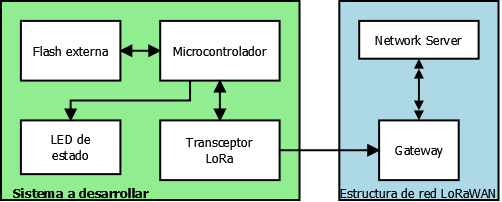
\includegraphics[width=.7\textwidth]{./Figuras/diagramaDeBloquesNivel1.png}
\caption{Diagrama en bloques del sistema}
\label{fig:diagBloquesNivel1}
\end{figure}

\vspace{25px}

Al entrar en el detalle del Transceptor LoRa, en la Figura \ref{fig:diagBloquesNivel2} se puede observar mejor los componentes del sistema. Existen tres partes importantes tanto del lado del servidor como del cliente. Estos bloques los define la recomendación técnica de la LoRa Alliance\textregistered. Los tres bloques son: Multicast usado para generar una ventana para la transmisión, Fragmentación que se encarga de fragmentar los paquetes a enviar y Sincornización de Relojes cuyo trabajo es asegurar la sincronización del dispositivo a actualizar con el sistema. Al rededor de ellos coexisten el Servidor de Actualización de Firmware que es el encargado de generar el firmware para la actualización. Tanto el servidor como el cliente están enlazados a través de un link LoRaWAN.

\vspace{25px}

\begin{figure}[htpb]
\centering 
\DIFdelbeginFL %DIFDELCMD < 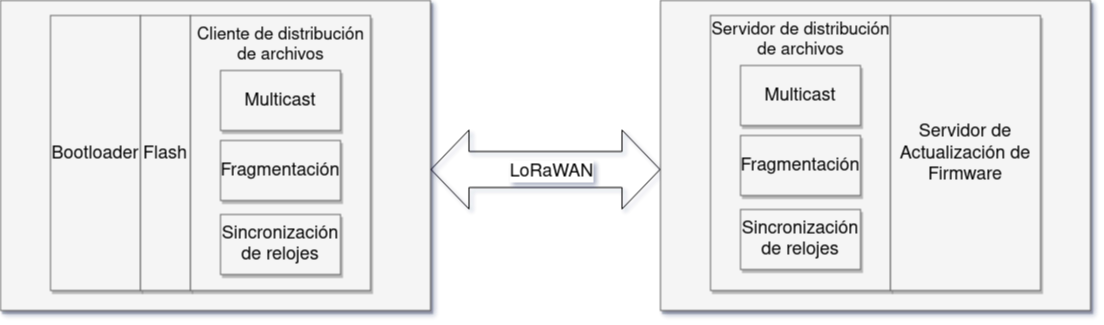
\includegraphics[width=.9\textwidth]{./Figuras/diagramaDeBloquesNivel2.png}
%DIFDELCMD < %%%
\DIFdelendFL \DIFaddbeginFL 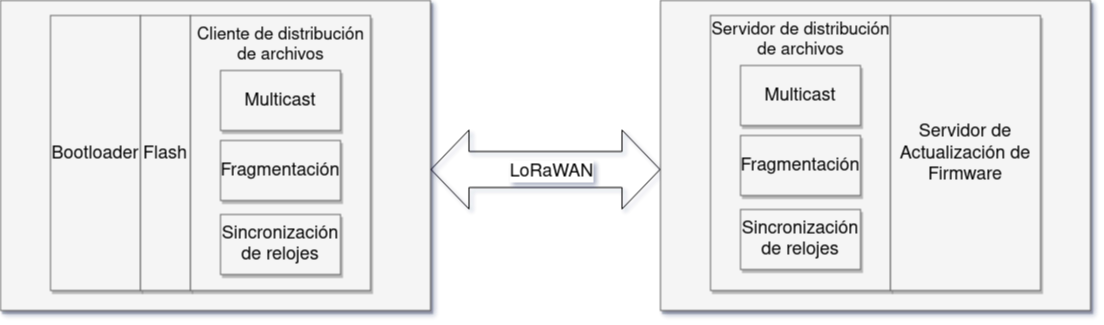
\includegraphics[width=\textwidth]{./Figuras/diagramaDeBloquesNivel2.png}
\DIFaddendFL \caption{Diagrama en bloques del sistema}
\label{fig:diagBloquesNivel2}
\end{figure}

\vspace{25px}


\end{consigna}


\section{Identificación y análisis de los interesados}
\label{sec:interesados}
A continuación se presentan los interesados involucrados en el desarrollo del proyecto.
\begin{consigna}{black} 
\begin{table}[ht]
%\caption{Identificación de los interesados}
%\label{tab:interesados}
\begin{tabularx}{\linewidth}{@{}|l|X|X|l|@{}}
\hline
\rowcolor[HTML]{C0C0C0} 
Rol           & Nombre y Apellido & Organización 	& Puesto 	\\ \hline
Cliente       & \clientename      &\empclientename	& Gerente de Ingeniería       	\\ \hline
Responsable   & \authorname       & FIUBA        	& Alumno 	\\ \hline
Colaboradores & Jhonattan Camargo &\empclientename  &Ingeniería de desarrollo \\ \hline
Orientador    & \supname	      & \pertesupname 	& Director	Trabajo final \\ \hline
Usuario final & Personal técnico o capacitado                  &              	&        	\\ \hline
\end{tabularx}
\end{table}

\begin{itemize}
\item Cliente: \clientename, Gerente de Ingeniería y el encargado del proyecto por parte de la empresa.
\item Colaborador: Jhonattan Camargo, Ingeniero en la empresa. Conocimiento técnico del proyecto y contacto directo ante cualquier duda.
\end{itemize}

\end{consigna}

\section{1. Propósito del proyecto}
\label{sec:proposito}

\begin{consigna}{black}
El proposito del proyecto es lograr un sistema que realice la actualización remota de firmware (FUOTA, por
sus siglas en inglés Firmware Update Over The Air) a través de una red LoRaWAN. El
dispositivo debe ser capaz de realizar la actualización a través de una memoria flash
externa en la que se guardarán las tramas recibidas \DIFdelbegin \DIFdel{inalambricamente}\DIFdelend \DIFaddbegin \DIFadd{inalámbricamente}\DIFaddend .
\end{consigna}

\section{2. Alcance del proyecto}
\label{sec:alcance}

\begin{consigna}{black}
El presente proyecto \DIFdelbegin \DIFdel{incluira}\DIFdelend \DIFaddbegin \DIFadd{incluirá}\DIFaddend :
\begin{itemize}
	\item Diseño de PCB del prototipo.
	\item Desarrollo de bootloader.
	\item Desarrollo de algoritmos para firma y verificación de firmware.
	\item Desarrollo de la fase de negociación de la ventana de distribución.
	\item Desarrollo de la fase fragmentación y ensamblaje de los paquetes a transmitir.
	\item Desarrollo de la fase de sincronización de relojes.
\end{itemize}

El presente proyecto no incluirá:
\begin{itemize}
	\item Desarrollo del servidor de red.
	\item Desarrollo del hardware a actualizar.
	\item Desarrollo de firmwares específicos.
	\item Desarrollo del gateway.
\end{itemize}

\end{consigna}


\section{3. Supuestos del proyecto}
\label{sec:supuestos}

\begin{consigna}{black}
Para el desarrollo del presente proyecto se supone que se cuenta con lo siguiente:

\begin{itemize}
\item Kits de desarrollo para \DIFdelbegin \DIFdel{LoraWAN}\DIFdelend \DIFaddbegin \DIFadd{LoRaWAN}\DIFaddend .
\item Hardware funcional que se usará para pruebas de actualización.
\item Gateway \DIFdelbegin \DIFdel{Lora}\DIFdelend \DIFaddbegin \DIFadd{LoRa}\DIFaddend .
\item Servidor donde correrán las aplicaciones.
\end{itemize}

La empresa también está comprometida a proveer espacios de trabajo si \DIFdelbegin \DIFdel{son }\DIFdelend \DIFaddbegin \DIFadd{fueran }\DIFaddend necesarios.
\end{consigna}

\section{4. Requerimientos}
\label{sec:requerimientos}
\begin{consigna}{black}
Los requerimientos funcionales y no funcionales del proyecto son los siguientes:
\begin{enumerate}
\item Requerimientos funcionales.
	\begin{enumerate}
	\item El sistema debe ser capaz de actualizar el firmware de un dispositvo usando la red LoRaWAN.
	\item El usuario debe ser capaz de elegir que dispositivo quiere actualizar.
	\item El usuario debe poder seleccionar el firmware a ser actualizado.
	\item El sistema debe permitir al usuario leer la versión del firmware en el dispositivo a ser actualizado.
	\item El sistema debe proveer una manera para asegurar la integridad del firmware.
	\item El sistema debe proveer al usuario opciones de firmado del firmware.
	\item El usuario debe estar en la capacidad de seleccionar la cantidad de fragmentos que se \DIFdelbegin \DIFdel{usaran }\DIFdelend \DIFaddbegin \DIFadd{usarán }\DIFaddend en la transmisión del firmware.
	\end{enumerate}
\item Requerimientos no funcionales.
	\begin{enumerate}
	\item Requerimientos del sistema.
	\begin{enumerate}
		\item El sistema debe basarse en las especificaciones establecidas por la LoRa Alliance\textregistered.
		\item El sistema debe usar una memoria externa para almacenar la actualización del firmware.
		\item La transmisión del firmware debe ser tolerante a fallas.
		\item El sistema usará dispositivos que aseguren el bajo consumo de energía.
		\item El software debe estar optimizado para lograr un equilibrio entre rendimiento y consumo de energía.
		\item El o los algoritmos usados deben asegurar la integridad y autenticidad del firmware a actualizar.
	\end{enumerate}
	\item Requerimientos de documentación
	\begin{itemize}
		\item Antes de comenzar el la implementación del proyecto debe existir un documento donde se contemple la planificación inicial.
		\item Se debe entregar una memoria donde se describa el diseño y funcionamiento del sistema.
	\end{itemize}
    \item Requerimientos de procesos
    \begin{itemize}
    	\item Se debe poder hacer una revisión del proyecto de manera semanal para poder hacer correcciones tempranas
    	\item Se usará un sistema de control de versión para el código y documentación del proyecto.
    \end{itemize}
	\end{enumerate}
\end{enumerate}

\end{consigna}

\DIFaddbegin \section{\DIFadd{Historias de usuarios (}\textit{\DIFadd{Product backlog}}\DIFadd{)}}
\label{sec:backlog}

\begin{consigna}{black}
\DIFadd{En las historias de usuario se consideran puntajes de 1 a 100 siendo 100 el número que representa el mayor esfuerzo. Hay historias como la planificación y el cumplimiento de las especificaciones que se consideran de mucho esfuerzo porque son transversales a todo el proyecto. 
}\begin{table}[htpb]
	\centering
	\begin{tabularx}{\linewidth}{@{}|X|c|@{}}
		\hline
		\rowcolor[HTML]{C0C0C0} 
		\multicolumn{2}{|c|}{\cellcolor[HTML]{C0C0C0}Historias de usuarios (\textit{Product Backlog})} \\ \hline
		\rowcolor[HTML]{C0C0C0} 
		\DIFaddFL{Descripción }&
		\multicolumn{1}{c|}{\cellcolor[HTML]{C0C0C0}Ponderación} \\ \hline
		\DIFaddFL{El cliente requiere la planificación del desarrollo. Sin esta planificación no se puede comenzar el proyecto ya que primero debe ser aprobada }& \DIFaddFL{100 }\\ \hline
		\DIFaddFL{Es necesario que el desarrollo cumpla con las especificaciones de la LoRa Alliance \textregistered. Si no cumple con este requerimiento, pueden haber problemas en cuanto a la funcionalidad }& \DIFaddFL{100 }\\ \hline
		\DIFaddFL{Un usuario debe poder usar el desarrollo después de una breve inducción así que se debe tener en cuenta esto al momento de diseñar la interacción con el usuario }& \DIFaddFL{20 }\\ \hline
		\DIFaddFL{El cliente demanda que el hardware debe ser aprobado antes de su fabricación. Esto implica la revisión da cada etapa de diseño }& \DIFaddFL{50 }\\ \hline
		\DIFaddFL{El cliente solicita que el desarrollo considere el bajo consumo de energía debido a que puede ser usado en zonas remotas donde puede haber problemas de electricidad }& \DIFaddFL{70 }\\ \hline
		\DIFaddFL{El usuario debe poder confiar en la transmisión del firmware. El usuario solicita que si hay un error en la transmisión del firmware, este no se actualice }& \DIFaddFL{50 }\\ \hline
		\DIFaddFL{El cliente solicita que el firmware este firmado para agregar seguridad }& \DIFaddFL{40 }\\ \hline
		\DIFaddFL{El usuario debe poder seleccionar la versión del firmware a actualizar }& \DIFaddFL{50}\\ \hline
		\DIFaddFL{El usuario debe poder elegir el dispositivo a actualizar }& \DIFaddFL{50 }\\ \hline
	\end{tabularx}%DIF > 
\end{table}


\end{consigna}

\DIFaddend \section{5. Entregables principales del proyecto}
\label{sec:entregables}

\begin{consigna}{black}
Los entregables del proyecto serán:
\begin{itemize}
\item Memoria descriptiva del proyecto.
\item Prototipo para la actualización del firmware.
\item Manual de utilización.
\item Diagramas esquemáticos.
\item Código fuente.

\end{itemize}

\end{consigna}

\section{6. Desglose del trabajo en tareas}
\label{sec:wbs}

\begin{consigna}{black}
Para la realización de este proyecto se consideran las siguientes tareas:

\begin{enumerate}
	\item Planificación. \hfill(62 hs)
	\begin{enumerate}
		\item Estudio de las \DIFdelbegin \DIFdel{especificacione. s }\DIFdelend \DIFaddbegin \DIFadd{especificaciones. }\DIFaddend \hfill(4 hs)
		\item Realización del documento de planificación. \hfill(15 hs)
		\item Revisión de la planificación. \hfill(3 hs)
		\item Reuniones semanales. \hfill(32 hs)
		\item Reuniones mensuales. \hfill(8 hs)
	\end{enumerate}
	\item Documentación bibliográfica e \DIFdelbegin \DIFdel{Investigación}\DIFdelend \DIFaddbegin \DIFadd{investigación}\DIFaddend . (75 hs)
	\begin{enumerate}
		\item Estudio del protocolo LoRa y LoRaWAN. \hfill(25 hs)
		\item Estudio de las \DIFdelbegin \DIFdel{especificaiones }\DIFdelend \DIFaddbegin \DIFadd{especificaciones }\DIFaddend de FUOTA de la LoRa Alliance\textregistered. \hfill(20 hs)
		\item Estudio de las soluciones existentes. \hfill(20 hs)
		\item Estudio de las especificaciones del hardware. \hfill(10 hs)
	\end{enumerate}
	\item Desarrollo del software. \hfill(210 hs)
	\begin{enumerate}
		\item Diseño de arquitectura. \hfill(20 hs)
		\item Pruebas de comunicación iniciales. \hfill(10 hs)
		\item Implementación de la fase de firma y verificación del firmware. \hfill(40 hs)
		\item Implementación de la fase de negociación de banda para la transmisión. \hfill(40 hs)
		\item Implementación de la fase de fragmentación y ensamblaje del firmware. \hfill(40 hs)
		\item Implementación de la fase de sincronización de relojes. \hfill(40 hs)
		\item Integración de los módulos del sistema. \hfill(20 hs)
	\end{enumerate}
    \item Desarrollo de hardware. \hfill(115 hs)
    \begin{enumerate}
    	\item Seleción de elementos constitutivos del prototipo. \hfill(5 hs)
    	\item Diseño de la arquitectura. \hfill(10 hs)
    	\item Diseño del diagrama esquemático. \hfill(30 hs)
    	\item Diseño del PCB. \hfill(30 hs)
    	\item Ensamblaje del prototipo. \hfill(40 hs)
    \end{enumerate}
	\item Pruebas \DIFdelbegin \DIFdel{en Integración}\DIFdelend \DIFaddbegin \DIFadd{de integración}\DIFaddend . \hfill(40 hs)
	\begin{enumerate}
		\item Pruebas de integración y funcionalidad. \hfill(40 hs)
	\end{enumerate}
	\item Documentación del proyecto. \hfill(100 hs)
	\begin{enumerate}
		\item Informe de de avance. \hfill(20 hs)
		\item Elaboración del manual del sistema. \hfill(20 hs)
		\item Memoria final del proyecto. \hfill(40 hs)
		\item Presentación final del proyecto. \hfill(20 hs)
	\end{enumerate}

\end{enumerate}

Cantidad total de horas: (602 hs).

\end{consigna}

\section{7. Diagrama de Activity On Node}
\label{sec:AoN}

\DIFdelbegin %DIFDELCMD < \begin{consigna}{red}
%DIFDELCMD < %%%
\DIFdel{Armar el AoN a partir del WBS definido en la etapa anterior. }%DIFDELCMD < 

%DIFDELCMD < %%%
%DIF < La figura \ref{fig:AoN} fue elaborada con el paquete latex tikz y pueden consultar la siguiente referencia \textit{online}:
%DIFDELCMD < 

%DIFDELCMD < %%%
%DIF < \url{https://www.overleaf.com/learn/latex/LaTeX_Graphics_using_TikZ:_A_Tutorial_for_Beginners_(Part_3)\%E2\%80\%94Creating_Flowcharts}
%DIFDELCMD < 

%DIFDELCMD < %%%
\DIFdelend \DIFaddbegin \begin{consigna}{black}
\DIFadd{En la figura \ref{fig:AoN} se puede observar el diagrama de Activity On Node. El camino crítico está resaltado. Todos los tiempos están en horas. En este diagrama no se presentan las horas usadas para las reuniones semanales y mensuales.
}\DIFaddend \end{consigna}

\DIFdelbegin %DIFDELCMD < \begin{figure}[htpb]
%DIFDELCMD < \centering 
%DIFDELCMD < 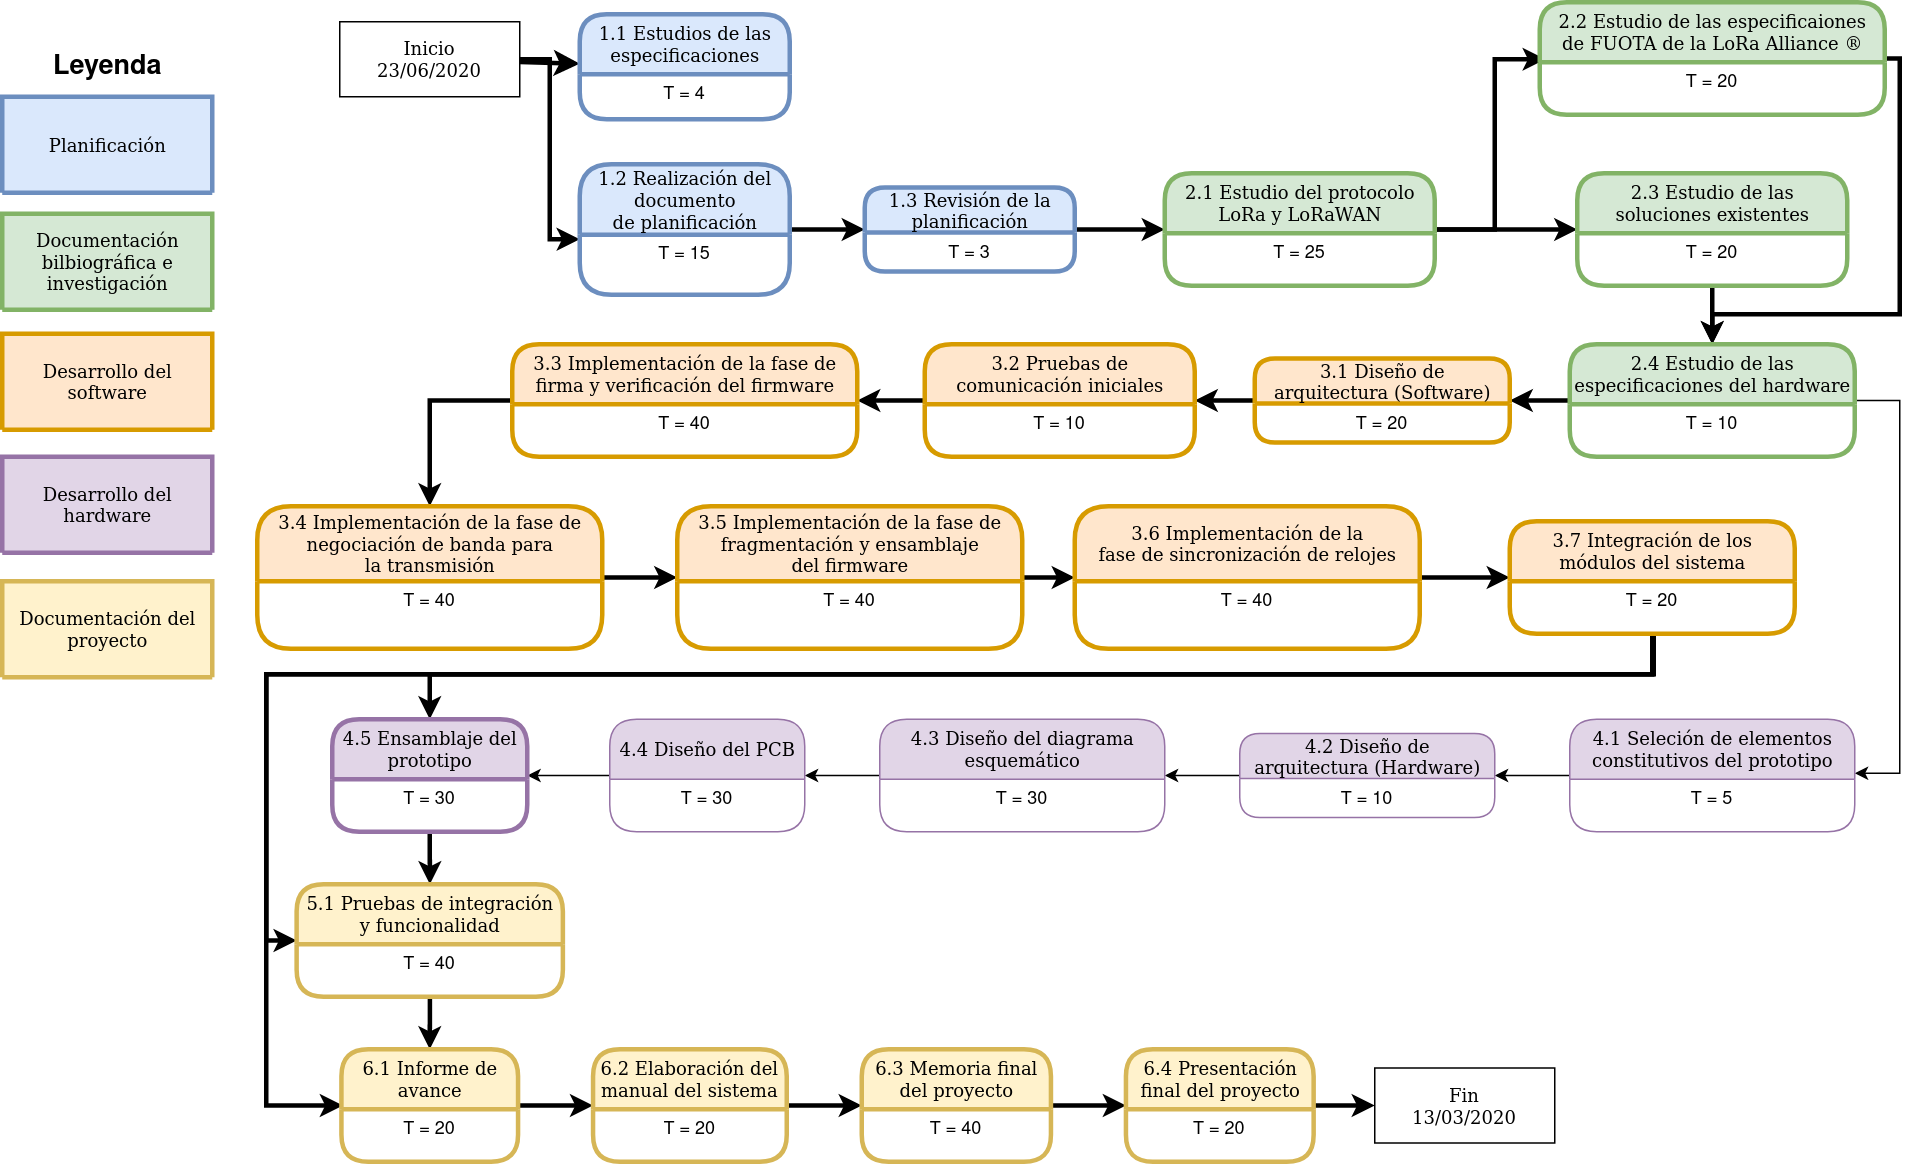
\includegraphics[width=.8\textwidth]{./Figuras/AoN.png}
%DIFDELCMD < %%%
%DIFDELCMD < \caption{%
{%DIFAUXCMD
\DIFdelFL{Diagrama en }\textit{\DIFdelFL{Activity on Node}}%DIFAUXCMD
}
%DIFAUXCMD
%DIFDELCMD < \label{fig:AoN}
%DIFDELCMD < \end{figure}
%DIFDELCMD < 

%DIFDELCMD < %%%
\DIFdel{Indicar claramente en qué unidades están expresados los tiempos. De ser necesario indicar los caminos semicríticos y analizar sus tiempos mediante un cuadro. Es recomendable usar colores y un cuadro indicativo describiendo qué representa cada color, como se muestra en el siguiente ejemplo:
}%DIFDELCMD < 

%DIFDELCMD < %%%
\DIFdelend \section{8. Diagrama de Gantt}
\label{sec:gantt}

\DIFdelbegin %DIFDELCMD < \begin{consigna}{red}
%DIFDELCMD < %%%
\DIFdel{Utilizar el software Gantter for Google Drive o alguno similar para dibujar el diagrama de Gantt.
}%DIFDELCMD < 

%DIFDELCMD < %%%
\DIFdel{Existen muchos programas y recursos }\textit{\DIFdel{online}} %DIFAUXCMD
\DIFdel{para hacer diagramas de gantt, entre las cuales destacamos:
}%DIFDELCMD < 

%DIFDELCMD < \begin{itemize}
\begin{itemize}%DIFAUXCMD
%DIFDELCMD < \item %%%
\item%DIFAUXCMD
\DIFdel{Planner
}%DIFDELCMD < \item %%%
\item%DIFAUXCMD
\DIFdel{GanttProject
}%DIFDELCMD < \item %%%
\item%DIFAUXCMD
\DIFdel{Trello + }\textit{\DIFdel{plugins}}%DIFAUXCMD
\DIFdel{. En el siguiente link hay un tutorial oficial: }%DIFDELCMD < \\ \url{https://blog.trello.com/es/diagrama-de-gantt-de-un-proyecto}
%DIFDELCMD < \item %%%
\item%DIFAUXCMD
\DIFdel{Creately, herramienta online colaborativa. }%DIFDELCMD < \\\url{https://creately.com/diagram/example/ieb3p3ml/LaTeX}
%DIFDELCMD < \item %%%
\item%DIFAUXCMD
\DIFdel{Se puede hacer en latex con el paquete }\textit{\DIFdel{pgfgantt}}%DIFAUXCMD
%DIFDELCMD < \\ \url{http://ctan.dcc.uchile.cl/graphics/pgf/contrib/pgfgantt/pgfgantt.pdf}

\end{itemize}%DIFAUXCMD
%DIFDELCMD < \end{itemize}
%DIFDELCMD < 

%DIFDELCMD < %%%
\DIFdel{Pegar acá una captura de pantalla del diagrama de Gantt, cuidando que la letra sea suficientemente grande como para ser legible. 
Si el diagrama queda demasiado ancho, se puede pegar primero la ``tabla'' del Gantt y luego pegar la parte del diagrama de barras del diagrama de Gantt .
}%DIFDELCMD < 

%DIFDELCMD < %%%
\DIFdel{Configurar el software para que en la parte de la tabla muestre los códigos del EDT (WBS). }%DIFDELCMD < \\
%DIFDELCMD < %%%
\DIFdel{Configurar el software para que al lado de cada barra muestre el nombre de cada tarea. }%DIFDELCMD < \\
%DIFDELCMD < %%%
\DIFdel{Revisar que }\DIFdelend \DIFaddbegin \begin{consigna}{black}
\DIFadd{En }\DIFaddend la \DIFaddbegin \DIFadd{figura \ref{fig:gantt} se observa el diagrama de Gantt del proyecto. Se considera que el tiempo de trabajo por semana es de 15 h. La finalización del trabajo no coincide con la }\DIFaddend fecha de finalización \DIFdelbegin \DIFdel{coincida con lo indicado en el Acta Constitutiva.
}\DIFdelend \DIFaddbegin \DIFadd{de la especialidad pero se podrá considerar extender esta fecha si las condiciones del trabajo lo requieren.
}\end{consigna}
\DIFaddend 

\DIFdelbegin \DIFdel{En la figura \ref{fig:gantt}, se muestra un ejemplo de diagrama de gantt realizado con el paquete de }\textit{\DIFdel{pgfgantt}}%DIFAUXCMD
\DIFdel{. En la plantilla pueden ver el código que lo genera y usarlo de base para construir el propio.
}%DIFDELCMD < 

%DIFDELCMD < \begin{figure}[htbp]
%DIFDELCMD < \begin{center}
%DIFDELCMD < \begin{ganttchart}{1}{12}
%DIFDELCMD <   \gantttitle{2020}{12} \\
%DIFDELCMD <   \gantttitlelist{1,...,12}{1} \\
%DIFDELCMD <   \ganttgroup{Group 1}{1}{7} \\
%DIFDELCMD <   \ganttbar{Task 1}{1}{2} \\
%DIFDELCMD <   \ganttlinkedbar{Task 2}{3}{7} \ganttnewline
%DIFDELCMD <   \ganttmilestone{Milestone o hito}{7} \ganttnewline
%DIFDELCMD <   \ganttbar{Final Task}{8}{12}
%DIFDELCMD <   \ganttlink{elem2}{elem3}
%DIFDELCMD <   \ganttlink{elem3}{elem4}
%DIFDELCMD < \end{ganttchart}
%DIFDELCMD < \end{center}
%DIFDELCMD < %%%
\DIFdelendFL \DIFaddbeginFL \begin{landscape}
	\begin{figure}
		\centering 
		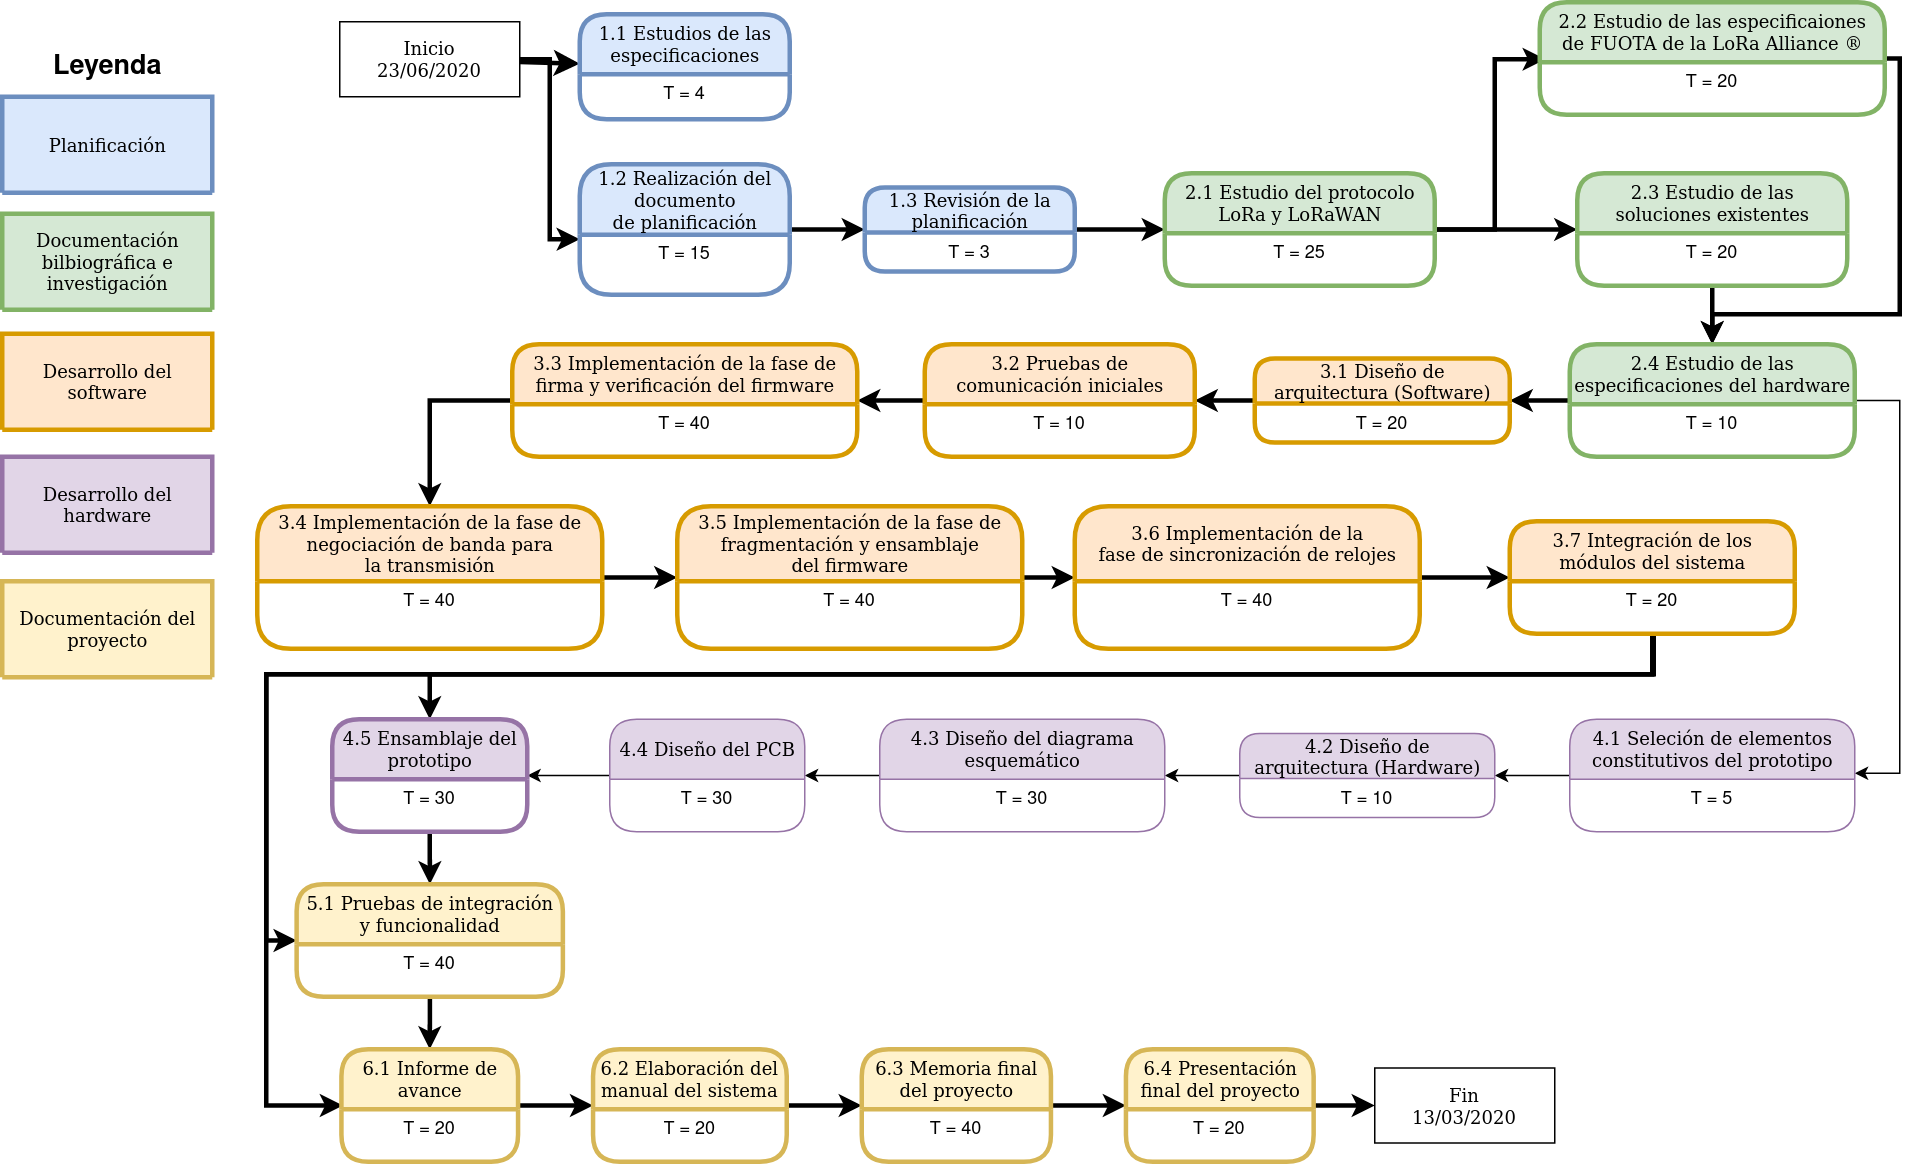
\includegraphics[width=20cm]{./Figuras/AoN.png}
		\DIFaddendFL \caption{Diagrama \DIFdelbeginFL \DIFdelFL{de gantt de ejemplo}\DIFdelendFL \DIFaddbeginFL \DIFaddFL{en }\textit{\DIFaddFL{Activity on Node}}\DIFaddendFL }
		\DIFaddbeginFL \label{fig:AoN}
	\end{figure}
\end{landscape}

\begin{landscape}
	\begin{figure}
		\centering 
		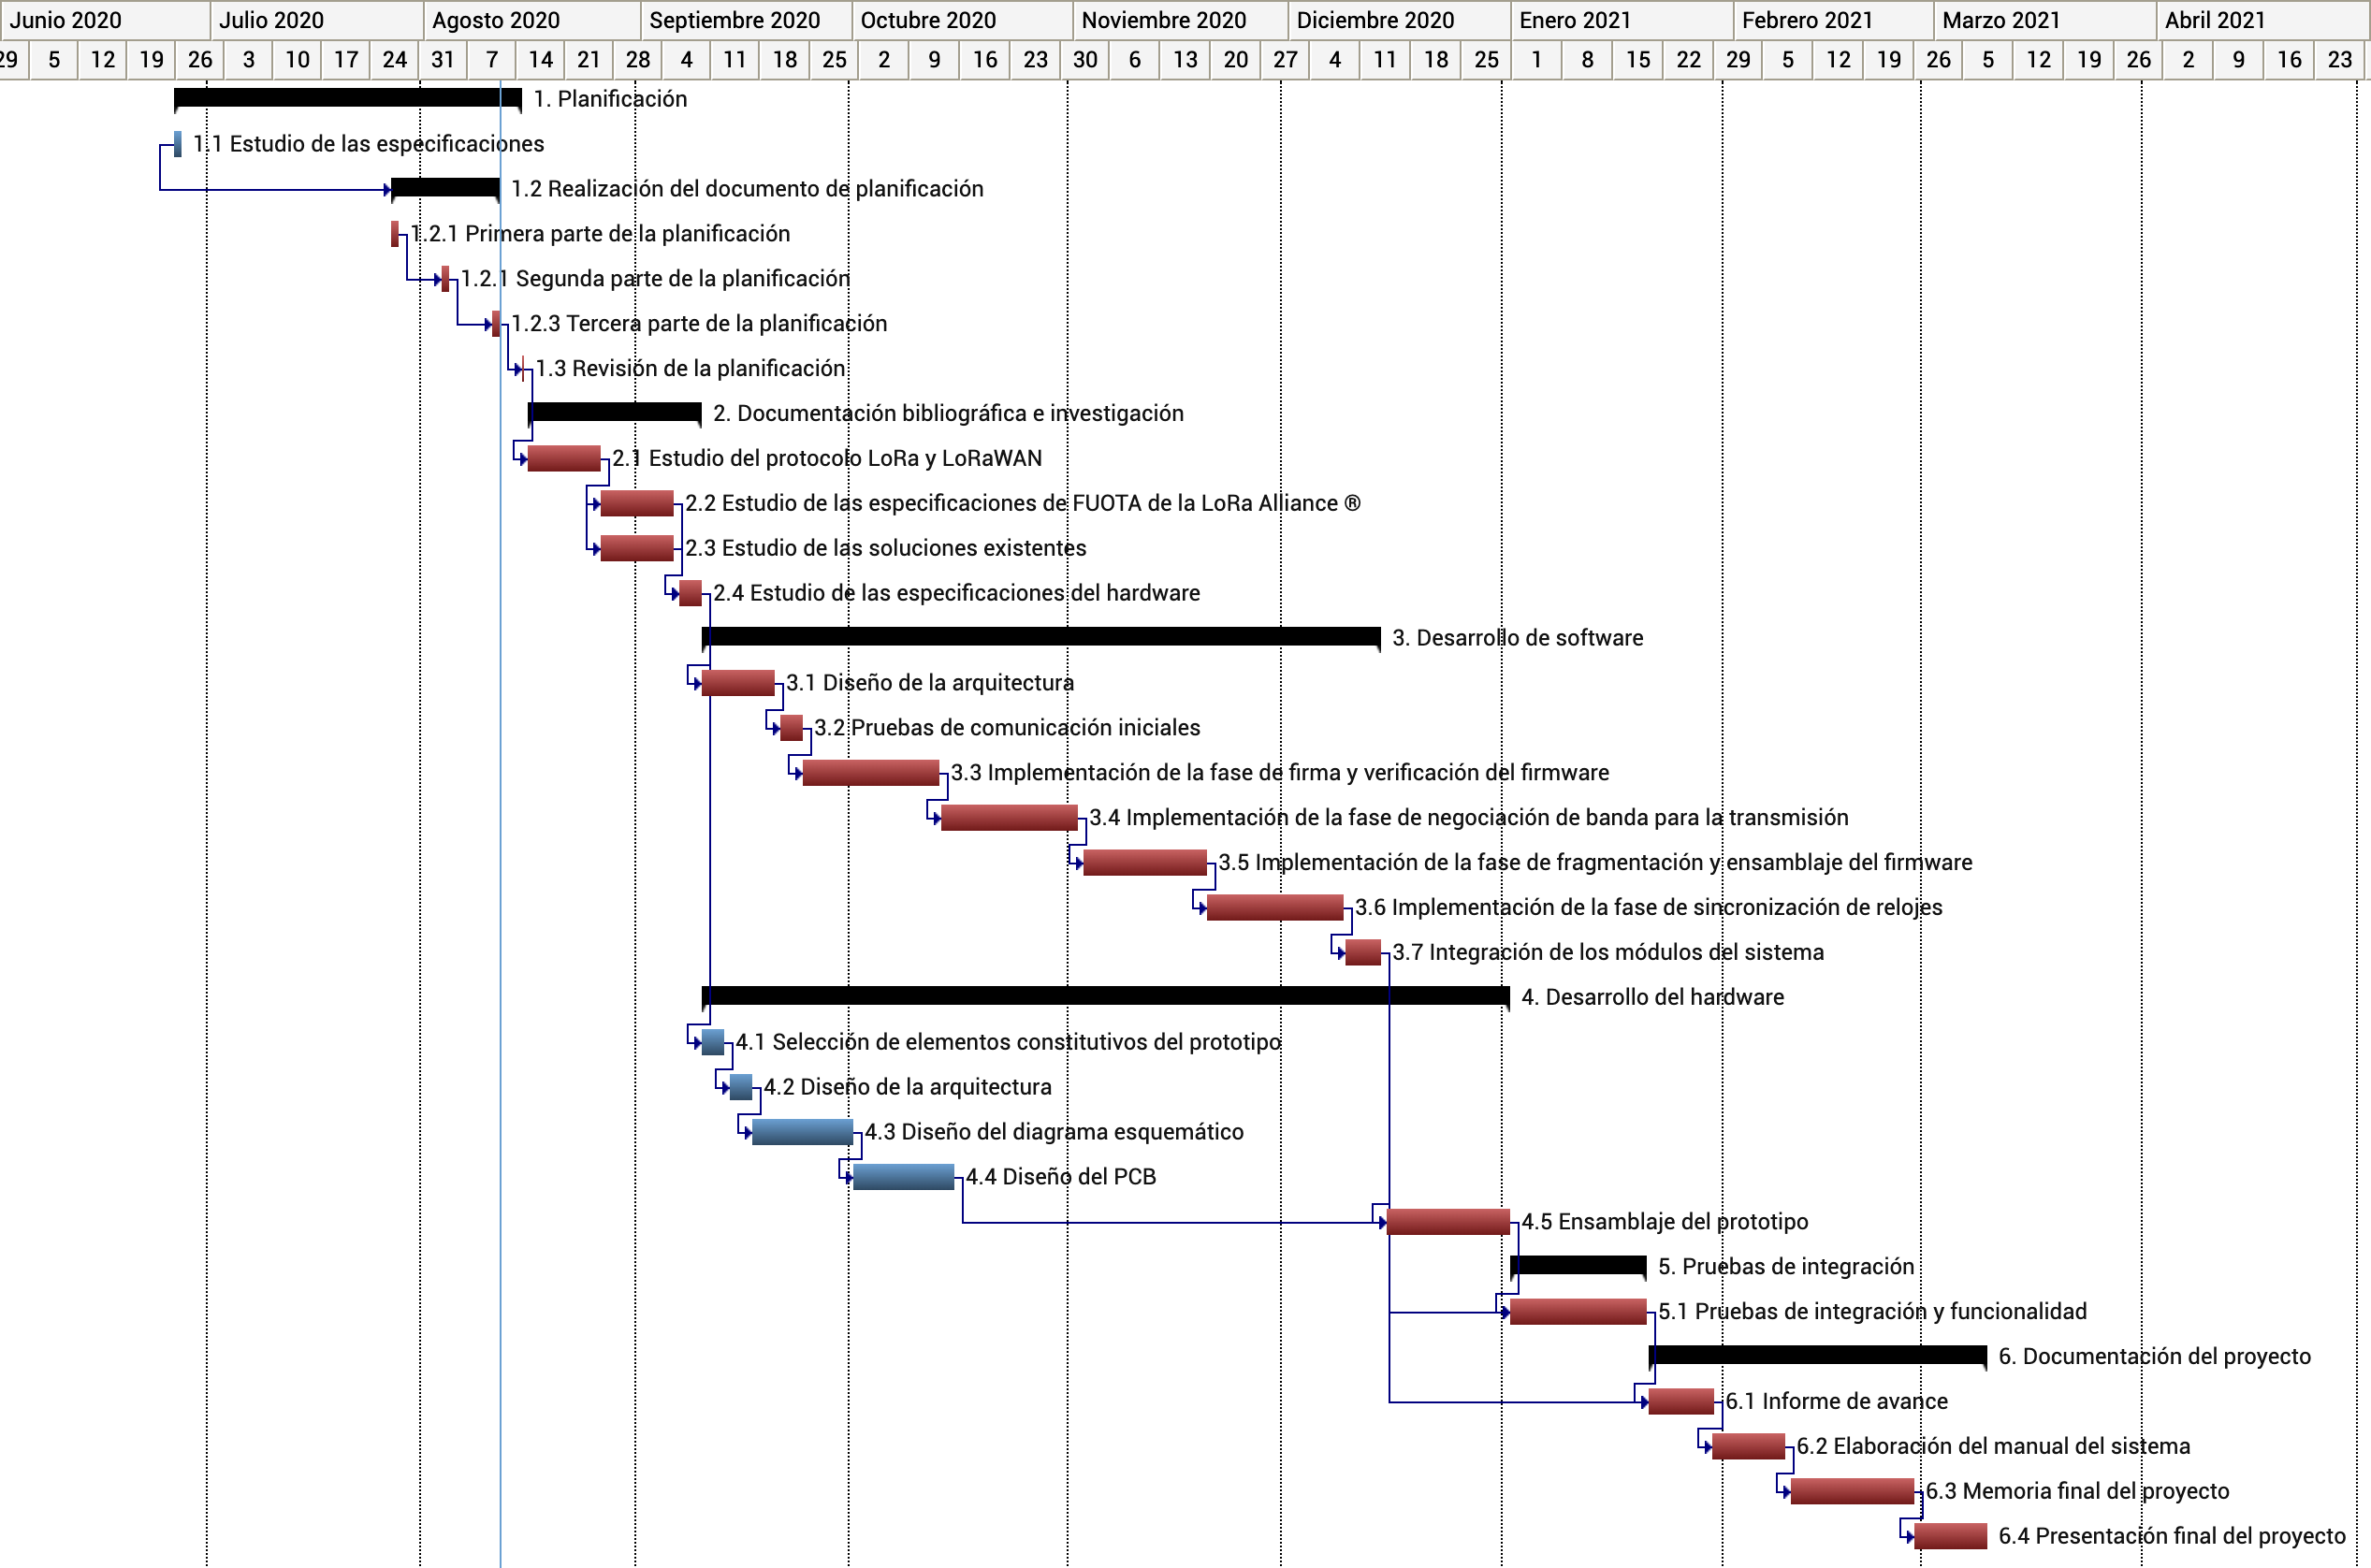
\includegraphics[width=20cm]{./Figuras/DiagramaGantt.png}
		\caption{\DIFaddFL{Diagrama de }\textit{\DIFaddFL{Gantt}}}
		\DIFaddendFL \label{fig:gantt}
	\end{figure}
\DIFaddbegin \end{landscape}
\DIFaddend 

\DIFdelbegin %DIFDELCMD < \end{consigna}
%DIFDELCMD < 

%DIFDELCMD < %%%
\DIFdelend \section{9. Matriz de uso de recursos de materiales}
\label{sec:recursos}

\DIFaddbegin \begin{consigna}{black}
	\DIFaddend \begin{table}[htpb]
		\label{tab:recursos}
		\centering
		\DIFdelbeginFL %DIFDELCMD < \begin{tabularx}{\linewidth}{@{}|c|X|X|X|X|X|@{}}
%DIFDELCMD < %%%
\DIFdelendFL \DIFaddbeginFL \begin{tabularx}{\linewidth}{@{}|c|X|c|c|c|c|@{}}
			\DIFaddendFL \hline
			\cellcolor[HTML]{C0C0C0} & \cellcolor[HTML]{C0C0C0} & \multicolumn{4}{c|}{\cellcolor[HTML]{C0C0C0}Recursos requeridos (horas)} \\ \cline{3-6} 
			\multirow{-2}{*}{\cellcolor[HTML]{C0C0C0}\begin{tabular}[c]{@{}c@{}}Código\\ WBS\end{tabular}} & \multirow{-2}{*}{\cellcolor[HTML]{C0C0C0}\begin{tabular}[c]{@{}c@{}}Nombre \\ tarea\end{tabular}} & \DIFdelbeginFL \DIFdelFL{Material }\DIFdelendFL \DIFaddbeginFL \DIFaddFL{Computador }& \begin{tabular}[t]{@{}c@{}}\DIFaddFL{Módulo xDOT }\\ \DIFaddFL{Development Kit}\end{tabular} & \begin{tabular}[t]{@{}c@{}}\DIFaddFL{Gateway}\\ \DIFaddFL{LoRa}\end{tabular} & \begin{tabular}[t]{@{}c@{}}\DIFaddFL{Prototipo}\\ \DIFaddFL{funcional}\end{tabular} \\ \hline
			\DIFaddendFL 1& \DIFdelbeginFL \DIFdelFL{Material }\DIFdelendFL \DIFaddbeginFL \DIFaddFL{Planificación }& \DIFaddFL{62 }&  &  &  \\ \hline
			\DIFaddendFL 2& \DIFdelbeginFL \DIFdelFL{Material 3 }\DIFdelendFL \DIFaddbeginFL \begin{tabular}[c]{@{}l@{}}\DIFaddFL{Documentación }\\ \DIFaddFL{bibliográfica e}\\ \DIFaddFL{investigación}\end{tabular} \DIFaddendFL & \DIFdelbeginFL \DIFdelFL{Material 4 }\DIFdelendFL \DIFaddbeginFL \DIFaddFL{75 }&  &  &  \DIFaddendFL \\ \hline
			\DIFaddbeginFL \DIFaddFL{3}\DIFaddendFL & \DIFaddbeginFL \DIFaddFL{Desarrollo del software }\DIFaddendFL & \DIFaddbeginFL \DIFaddFL{210 }\DIFaddendFL & \DIFaddbeginFL \DIFaddFL{170 }\DIFaddendFL & \DIFaddbeginFL \DIFaddFL{170 }\DIFaddendFL &  \\ \hline
			\DIFaddbeginFL \DIFaddFL{4}\DIFaddendFL & \DIFaddbeginFL \DIFaddFL{Desarrollo del hardware }\DIFaddendFL & \DIFaddbeginFL \DIFaddFL{115 }\DIFaddendFL &  &  &  \\ \hline
			\DIFaddbeginFL \DIFaddFL{5}\DIFaddendFL & \DIFaddbeginFL \DIFaddFL{Pruebas de integración }\DIFaddendFL & \DIFaddbeginFL \DIFaddFL{40 }\DIFaddendFL &  &  & \DIFaddbeginFL \DIFaddFL{40 }\DIFaddendFL \\ \hline
			\DIFaddbeginFL \DIFaddFL{6}\DIFaddendFL & \DIFaddbeginFL \DIFaddFL{Documentación del proyecto }\DIFaddendFL & \DIFaddbeginFL \DIFaddFL{100 }\DIFaddendFL &  &  &  \\ \hline
		\end{tabularx}%
	\end{table}

\DIFaddbegin \end{consigna}

\DIFaddend \section{10. Presupuesto detallado del proyecto}
\label{sec:presupuesto}

\DIFdelbegin %DIFDELCMD < \begin{consigna}{red}
%DIFDELCMD < %%%
\DIFdel{Si el proyecto es complejo entonces separarlo en partes:
}%DIFDELCMD < \begin{itemize}
\begin{itemize}%DIFAUXCMD
%DIFDELCMD < \item %%%
\item%DIFAUXCMD
\DIFdel{Un total global, indicando el subtotal acumulado por cada una de las áreas.
}%DIFDELCMD < \item %%%
\item%DIFAUXCMD
\DIFdel{El desglose detallado del subtotal de cada una de las áreas.
}
\end{itemize}%DIFAUXCMD
%DIFDELCMD < \end{itemize}
%DIFDELCMD < %%%
\DIFdelend \DIFaddbegin \begin{consigna}{black}
\DIFaddend 

\DIFdelbegin \DIFdel{IMPORTANTE: No olvidarse de considerar los COSTOS INDIRECTOS.
}%DIFDELCMD < 

%DIFDELCMD < \end{consigna}
%DIFDELCMD < 

%DIFDELCMD < %%%
\DIFdelend \begin{table}[htpb]
	\centering
	\begin{tabularx}{\linewidth}{@{}|X|c|r|r|@{}}
		\hline
		\rowcolor[HTML]{C0C0C0} 
		\multicolumn{4}{|c|}{\cellcolor[HTML]{C0C0C0}COSTOS DIRECTOS} \\ \hline
		\rowcolor[HTML]{C0C0C0} 
		Descripción &
		\multicolumn{1}{c|}{\cellcolor[HTML]{C0C0C0}Cantidad} &
		\multicolumn{1}{c|}{\cellcolor[HTML]{C0C0C0}Valor unitario} &
		\multicolumn{1}{c|}{\cellcolor[HTML]{C0C0C0}Valor total} \\ \hline
		\DIFaddbeginFL \DIFaddFL{Horas de ingeniería}\DIFaddendFL & \DIFdelbeginFL %DIFDELCMD < \multicolumn{1}{c|}{} %%%
\DIFdelendFL \DIFaddbeginFL \DIFaddFL{602 }\DIFaddendFL & \DIFdelbeginFL %DIFDELCMD < \multicolumn{1}{c|}{} %%%
\DIFdelendFL \DIFaddbeginFL \DIFaddFL{800 }\DIFaddendFL & \DIFdelbeginFL %DIFDELCMD < \multicolumn{1}{c|}{} %%%
\DIFdelendFL \DIFaddbeginFL \DIFaddFL{481600 }\DIFaddendFL \\ \hline
		\DIFaddbeginFL \DIFaddFL{Módulo xDOT Development Kit}\DIFaddendFL & \DIFdelbeginFL %DIFDELCMD < \multicolumn{1}{c|}{} %%%
\DIFdelendFL \DIFaddbeginFL \DIFaddFL{1 }\DIFaddendFL & \DIFdelbeginFL %DIFDELCMD < \multicolumn{1}{c|}{} %%%
\DIFdelendFL \DIFaddbeginFL \DIFaddFL{11400 }\DIFaddendFL & \DIFdelbeginFL %DIFDELCMD < \multicolumn{1}{c|}{} %%%
\DIFdelendFL \DIFaddbeginFL \DIFaddFL{11400 }\DIFaddendFL \\ \hline
		\DIFdelbeginFL %DIFDELCMD < \multicolumn{1}{|l|}{} %%%
\DIFdelendFL \DIFaddbeginFL \DIFaddFL{Fabricación de PCB }\DIFaddendFL & \DIFaddbeginFL \DIFaddFL{5 }\DIFaddendFL & \DIFaddbeginFL \DIFaddFL{1200 }\DIFaddendFL & \DIFaddbeginFL \DIFaddFL{6000 }\DIFaddendFL \\ \hline
		\DIFdelbeginFL %DIFDELCMD < \multicolumn{1}{|l|}{} %%%
\DIFdelendFL \DIFaddbeginFL \DIFaddFL{Ensamblaje de prototipo }\DIFaddendFL & \DIFaddbeginFL \DIFaddFL{5 }\DIFaddendFL & \DIFaddbeginFL \DIFaddFL{2420 }\DIFaddendFL & \DIFaddbeginFL \DIFaddFL{12100 }\DIFaddendFL \\ \hline
		\DIFaddbeginFL \DIFaddFL{Infraestructura en Amazon AWS }& \DIFaddFL{- }& \DIFaddFL{- }& \DIFaddFL{17800 }\\ \hline
		\DIFaddendFL \multicolumn{3}{|c|}{SUBTOTAL} &
		\DIFdelbeginFL %DIFDELCMD < \multicolumn{1}{c|}{} %%%
\DIFdelendFL \DIFaddbeginFL \multicolumn{1}{r|}{528900} \DIFaddendFL \\ \hline
		\rowcolor[HTML]{C0C0C0} 
		\multicolumn{4}{|c|}{\cellcolor[HTML]{C0C0C0}COSTOS INDIRECTOS} \\ \hline
		\rowcolor[HTML]{C0C0C0} 
		Descripción &
		\multicolumn{1}{c|}{\cellcolor[HTML]{C0C0C0}Cantidad} &
		\multicolumn{1}{c|}{\cellcolor[HTML]{C0C0C0}Valor unitario} &
		\multicolumn{1}{c|}{\cellcolor[HTML]{C0C0C0}Valor total} \\ \hline
		\DIFdelbeginFL %DIFDELCMD < \multicolumn{1}{|l|}{} %%%
\DIFdelendFL \DIFaddbeginFL \multicolumn{1}{|l|}{30 \% de los costos directos} \DIFaddendFL &
		\DIFaddbeginFL \DIFaddFL{1}\DIFaddendFL &
		\DIFaddbeginFL \DIFaddFL{158670}\DIFaddendFL &
		\DIFaddbeginFL \DIFaddFL{158670}\DIFaddendFL \\ \hline
		\DIFdelbeginFL %DIFDELCMD < \multicolumn{1}{|l|}{} &
%DIFDELCMD <    &
%DIFDELCMD <    &
%DIFDELCMD <    \\ \hline
%DIFDELCMD < \multicolumn{1}{|l|}{} &
%DIFDELCMD <    &
%DIFDELCMD <    &
%DIFDELCMD <    \\ \hline
%DIFDELCMD < %%%
\DIFdelendFL \multicolumn{3}{|c|}{SUBTOTAL} &
		\DIFdelbeginFL %DIFDELCMD < \multicolumn{1}{c|}{} %%%
\DIFdelendFL \DIFaddbeginFL \multicolumn{1}{r|}{158670} \DIFaddendFL \\ \hline
		\rowcolor[HTML]{C0C0C0}
		\multicolumn{3}{|c|}{TOTAL} &
		\DIFaddbeginFL \DIFaddFL{687570}\DIFaddendFL \\ \hline
	\end{tabularx}%
\end{table}

\DIFaddbegin \end{consigna}


\DIFaddend \section{11. Matriz de asignación de responsabilidades}
\label{sec:responsabilidades}
\DIFdelbegin %DIFDELCMD < \begin{consigna}{red}
%DIFDELCMD < %%%
\DIFdel{Establecer la matriz de asignación de responsabilidades y el manejo de la autoridad completando la siguiente tabla:
}%DIFDELCMD < 

%DIFDELCMD < %%%
\DIFdelend \DIFaddbegin \begin{consigna}{black}
\DIFaddend \begin{table}[htpb]
\centering
\DIFdelbeginFL %DIFDELCMD < \resizebox{\textwidth}{!}{%
%DIFDELCMD < \begin{tabular}{|c|c|c|c|c|c|}
%DIFDELCMD < \hline
%DIFDELCMD < \rowcolor[HTML]{C0C0C0} 
%DIFDELCMD < \cellcolor[HTML]{C0C0C0} &
%DIFDELCMD <   \cellcolor[HTML]{C0C0C0} &
%DIFDELCMD <   \multicolumn{4}{c|}{\cellcolor[HTML]{C0C0C0}Listar todos los nombres y roles del proyecto} \\ \cline{3-6} 
%DIFDELCMD < \rowcolor[HTML]{C0C0C0} 
%DIFDELCMD < \cellcolor[HTML]{C0C0C0} &
%DIFDELCMD <   \cellcolor[HTML]{C0C0C0} &
%DIFDELCMD <   Responsable &
%DIFDELCMD <   Orientador &
%DIFDELCMD <   Equipo &
%DIFDELCMD <   Cliente \\ \cline{3-6} 
%DIFDELCMD < \rowcolor[HTML]{C0C0C0} 
%DIFDELCMD < \multirow{-3}{*}{\cellcolor[HTML]{C0C0C0}\begin{tabular}[c]{@{}c@{}}Código\\ WBS\end{tabular}} &
%DIFDELCMD <   \multirow{-3}{*}{\cellcolor[HTML]{C0C0C0}Nombre de la tarea} &
%DIFDELCMD <   \authorname &
%DIFDELCMD <   \supname &
%DIFDELCMD <   Nombre de alguien &
%DIFDELCMD <   \clientename \\ \hline
%DIFDELCMD <  &  &  &  &  &  \\ \hline
%DIFDELCMD <  &  &  &  &  &  \\ \hline
%DIFDELCMD <  &  &  &  &  &  \\ \hline
%DIFDELCMD < \end{tabular}%
%DIFDELCMD < }
%DIFDELCMD < %%%
\DIFdelendFL \DIFaddbeginFL \resizebox{\linewidth}{!}{%
\begin{tabular}{|c|c|c|c|c|c|}
\hline
\rowcolor[HTML]{C0C0C0} 
\cellcolor[HTML]{C0C0C0} &
  \cellcolor[HTML]{C0C0C0} &
  \multicolumn{4}{c|}{\cellcolor[HTML]{C0C0C0}Listar todos los nombres y roles del proyecto} \\ \cline{3-6} 
\rowcolor[HTML]{C0C0C0} 
\cellcolor[HTML]{C0C0C0} &
  \cellcolor[HTML]{C0C0C0} &
  Responsable &
  Orientador &
  Equipo &
  Cliente \\ \cline{3-6} 
\rowcolor[HTML]{C0C0C0} 
\multirow{-3}{*}{\cellcolor[HTML]{C0C0C0}\begin{tabular}[c]{@{}c@{}}Código\\ WBS\end{tabular}} &
  \multirow{-3}{*}{\cellcolor[HTML]{C0C0C0}Nombre de la tarea} &
  \authorname &
  \supname &
  \cosupname &
  \clientename \\ \hline
 1.1 & Estudio de las especificaciones & P &  &  &  \\ \hline
 1.2 & Realización del documento de planificación & P & A & A & A \\ \hline
 1.3 & Revisión de la planificación &  & P & S &  \\ \hline
 1.4 & Reuniones semanales & P & P & P & P \\ \hline
 1.5 & Reuniones mensuales & P & P & P & P \\ \hline
 2.1 & Estudio del protocolo LoRa y LoRaWAN & P &  & C &  \\ \hline
 2.2 & Estudio de las especificaciones de FUOTA de la LoRa Alliance \textregistered & P &  & C &  \\ \hline
 2.3 & Estudio de las soluciones existentes & P &  & C &  \\ \hline
 2.4 & Estudio de las especificaciones del hardware & P &  &  &  \\ \hline
 3.1 & Diseño de arquitectura & P & A & C & A \\ \hline
 3.2 & Pruebas de comunicación iniciales & P &  & C &  \\ \hline
 3.3 & Implementación de la fase de firma y verificación del firmware & P & A & C & A \\ \hline
 3.4 & Implementación de la fase de negociación de banda para la transmisión & P & A & C & A \\ \hline
 3.5 & Implementación de la fase de fragmentación y ensamblaje del firmware & P & A & C & A \\ \hline
 3.6 & Implementación de la fase de sincronización de relojes & P & A & C & A \\ \hline
 3.7 & Integración de los módulos del sistema & P & A & C & A \\ \hline
 4.1 & Seleción de elementos constitutivos del prototipo & P & A & C & A \\ \hline
 4.2 & Diseño de la arquitectura & P & A & C & A \\ \hline
 4.3 & Diseño del diagrama esquemático & P & A & C & A \\ \hline
 4.4 & Diseño del PCB & P &  & C &  \\ \hline
 4.5 & Ensamblaje del prototipo & P & I & C & I \\ \hline
 5.1 & Pruebas de integración y funcionalidad & P & I & C & I \\ \hline
 6.1 & Informe de de avance & P & A & A & A \\ \hline
 6.2 & Elaboración del manual del sistema & P & A & A & A \\ \hline
 6.3 & Memoria final del proyecto & P & A & A & A \\ \hline
 6.4 & Presentación final del proyecto & P & A & A & A \\ \hline
\end{tabular}%
}
\DIFaddendFL \end{table}

{\footnotesize
Referencias:
\begin{itemize}
	\item P = Responsabilidad Primaria
	\item S = Responsabilidad Secundaria
	\item A = Aprobación
	\item I = Informado
	\item C = Consultado
\end{itemize}
} %footnotesize
\DIFdelbegin %DIFDELCMD < 

%DIFDELCMD < %%%
\DIFdel{Una de las columnas debe ser para el Director, ya que se supone que participará en el proyecto.
A su vez se debe cuidar que no queden muchas tareas seguidas sin ``A'' o ``I''.
}%DIFDELCMD < 

%DIFDELCMD < %%%
\DIFdel{Importante: es redundante poner ``I/A'' o ``I/C'', porque para aprobarlo o responder consultas primero la persona debe ser informada.
}%DIFDELCMD < 

%DIFDELCMD < %%%
\DIFdelend \end{consigna}

\section{12. Gestión de riesgos}
\label{sec:riesgos}

\DIFdelbegin %DIFDELCMD < \begin{consigna}{red}
%DIFDELCMD < %%%
\DIFdelend \DIFaddbegin \begin{consigna}{black}
\DIFaddend a) Identificación de los riesgos (al menos cinco) y estimación de sus consecuencias:

Riesgo 1: \DIFdelbegin \DIFdel{detallar el riesgo (riesgo es algo que si ocurre altera los planes previstos)
}\DIFdelend \DIFaddbegin \DIFadd{Problemas en la integración de los módulos de software.
}\DIFaddend \begin{itemize}
	\item Severidad (S) \DIFdelbegin \DIFdel{: mientras más severo, más alto es el número (usar números del 1 al 10).
	}%DIFDELCMD < \\
%DIFDELCMD < %%%
\DIFdel{Justificar el motivo por el cual se asigna determinado número de severidad }\DIFdelend \DIFaddbegin \DIFadd{9: La integración, al ser el paso final del desarrollo de software, puede presentar porblemas debido a problemas en la implementación de los módulos.
	}\item \DIFadd{Ocurrencia (O) 3: La probabilidad de ocurrencia se basa en que el proceso de desarrollo puede presentar problemas que se verán al momento de la integración.
}\end{itemize}

\DIFadd{Riesgo 2: Problemas relacionados con el servidor de red LoRaWAN.
}\begin{itemize}
	\item \DIFadd{Severidad }\DIFaddend (S) \DIFaddbegin \DIFadd{8: LoRaWAN necesita un servidor red para su funcionamiento. Si este servidor falla, las actualizaciones a los dispositivos no se entregarán}\DIFaddend .
	\item \DIFdelbegin \DIFdel{Probabilidad de ocurrencia }\DIFdelend \DIFaddbegin \DIFadd{Ocurrencia }\DIFaddend (O) \DIFdelbegin \DIFdel{: mientras más probable, más alto es el número (usar del 1 al 10) .}%DIFDELCMD < \\
%DIFDELCMD < %%%
\DIFdel{Justificar el motivo por el cual se asigna determinado número de }\DIFdelend \DIFaddbegin \DIFadd{2: La ocurrencia se considera baja porque se planea configurar el servidor en servicos de AWS. Se considera que los servicios de la nube son de alta confiabilidad.
}\end{itemize}

\DIFadd{Riesgo 3: Calidad de los entregables propuestos en el poryecto.
}\begin{itemize}
	\item \DIFadd{Severidad (S) 10: Si los entregables no cumplen con las expectativas de calidad de la empresa, el producto no podrá ponerse en producción. Esto ocasionaría una pérdidad de tiempo y dinero importante.
	}\item \DIFadd{Ocurrencia }\DIFaddend (O) \DIFaddbegin \DIFadd{4: Aunque se seguirán estándares de calidad en el diseño, existe una probabilidad considerable que los entregables no cumplan con las espcificaciones de calidad del cliente}\DIFaddend .
\end{itemize}

Riesgo \DIFdelbegin \DIFdel{2: }\DIFdelend \DIFaddbegin \DIFadd{4: Problemas para conseguir los elementos que constituyen el hardware.
}\DIFaddend \begin{itemize}
	\item Severidad (S) \DIFdelbegin \DIFdel{: 
}\DIFdelend \DIFaddbegin \DIFadd{10: Este severidad se considera uy alta porque impediría la elaboración del prototipo.
	}\DIFaddend \item Ocurrencia (O) \DIFdelbegin \DIFdel{:
}\DIFdelend \DIFaddbegin \DIFadd{1: La ocurrencia es baja porque l Mtor parte de los elemntos están presentes en el país, además la empresa auspiciante tiene experiencia en la importación de partes.
}\DIFaddend \end{itemize}

Riesgo \DIFdelbegin \DIFdel{3: }\DIFdelend \DIFaddbegin \DIFadd{5: Problemas en el ensamblaje del prototipo.
}\DIFaddend \begin{itemize}
	\item Severidad (S) \DIFdelbegin \DIFdel{: 
}\DIFdelend \DIFaddbegin \DIFadd{9: Si el prototipo presenta problemas en el ensamblaje no se pueden hacer pruebas de integración. Este es uno de los entregables más importantes.
	}\DIFaddend \item Ocurrencia (O) \DIFdelbegin \DIFdel{:
}\DIFdelend \DIFaddbegin \DIFadd{5: Esta ocurrencia puede ser alta por la inexperiencia que puede haber en el momento del ensamblaje.
}\DIFaddend \end{itemize}

b) Tabla de gestión de riesgos:      
\DIFdelbegin \DIFdel{(El RPN }\DIFdelend \DIFaddbegin 

\DIFadd{El $RPN$ }\DIFaddend se calcula como \DIFdelbegin \DIFdel{RPN=SxO)
}\DIFdelend \DIFaddbegin \DIFadd{$RPN=S \times O$. Si el $RPN$ sobrepasa el valor de 25, se tomarán medidas de mitigación.
}\DIFaddend 

\DIFdelbegin %DIFDELCMD < \begin{table}[htpb]
%DIFDELCMD < %%%
\DIFdelendFL \DIFaddbeginFL \begin{table}[H]
\DIFaddendFL \centering
\begin{tabularx}{\linewidth}{@{}|X|c|c|c|c|c|c|@{}}
\hline
\rowcolor[HTML]{C0C0C0} 
Riesgo & S & O & RPN & S* & O* & RPN* \\ \hline
\DIFaddbeginFL \DIFaddFL{Problemas en la integración de los módulos de software       }\DIFaddendFL & \DIFaddbeginFL \DIFaddFL{9  }\DIFaddendFL & \DIFaddbeginFL \DIFaddFL{3  }\DIFaddendFL &   \DIFaddbeginFL \DIFaddFL{27  }\DIFaddendFL & \DIFaddbeginFL \DIFaddFL{9   }\DIFaddendFL & \DIFaddbeginFL \DIFaddFL{2   }\DIFaddendFL &  \DIFaddbeginFL \DIFaddFL{18    }\DIFaddendFL \\ \hline
\DIFaddbeginFL \DIFaddFL{Problemas relacionados con el servidor de red LoRaWAN }\DIFaddendFL & \DIFaddbeginFL \DIFaddFL{8 }\DIFaddendFL & \DIFaddbeginFL \DIFaddFL{2 }\DIFaddendFL & \DIFaddbeginFL \DIFaddFL{16 }\DIFaddendFL & & & \\ \hline
\DIFaddbeginFL \DIFaddFL{Calidad de los entregables propuestos en el poryecto }\DIFaddendFL & \DIFaddbeginFL \DIFaddFL{10 }\DIFaddendFL & \DIFaddbeginFL \DIFaddFL{4 }\DIFaddendFL & \DIFaddbeginFL \DIFaddFL{40 }\DIFaddendFL & \DIFaddbeginFL \DIFaddFL{10  }\DIFaddendFL & \DIFaddbeginFL \DIFaddFL{1 }\DIFaddendFL &  \DIFaddbeginFL \DIFaddFL{10 }\DIFaddendFL \\ \hline
 \DIFaddbeginFL \DIFaddFL{Problemas para conseguir los elementos que constituyen el hardware      }\DIFaddendFL & \DIFaddbeginFL \DIFaddFL{10  }\DIFaddendFL &  \DIFaddbeginFL \DIFaddFL{1 }\DIFaddendFL &  \DIFaddbeginFL \DIFaddFL{10   }\DIFaddendFL &    &    &     \\ \hline
\DIFaddbeginFL \DIFaddFL{Problemas en el ensamblaje del prototipo }\DIFaddendFL & \DIFaddbeginFL \DIFaddFL{9  }\DIFaddendFL & \DIFaddbeginFL \DIFaddFL{5  }\DIFaddendFL &  \DIFaddbeginFL \DIFaddFL{45   }\DIFaddendFL &  \DIFaddbeginFL \DIFaddFL{9  }\DIFaddendFL &  \DIFaddbeginFL \DIFaddFL{2  }\DIFaddendFL &  \DIFaddbeginFL \DIFaddFL{18    }\DIFaddendFL \\ \hline
\end{tabularx}%
\end{table}

\DIFdelbegin \DIFdel{Criterio adoptado: 
Se tomarán medidas de mitigación en los riesgos cuyos números de RPN sean mayores a ....
}%DIFDELCMD < 

%DIFDELCMD < %%%
\DIFdel{Nota: los valores marcados con (*) en la tabla corresponden luego de haber aplicado la mitigación.
}%DIFDELCMD < 

%DIFDELCMD < %%%
\DIFdelend c) Plan de mitigación de los riesgos que originalmente excedían el RPN máximo establecido:

 Riesgo 1: \DIFdelbegin \DIFdel{Plan de }\DIFdelend \DIFaddbegin \DIFadd{Para mitigar este problema, se intentará hacer el diseño siguiendo una aproximación al diseño de software guiado por tests.
 }\begin{itemize}
 	\item \DIFadd{Severidad (S) 9: Se mantiene porque los problemas en la integración se traducen en que el sistema no funcionaría como un todo.
 	}\item \DIFadd{Ocurrencia (O) 2: Disminuye porque cada módulo será testeado para determinar su funcionamineto. Cada test debe cumplir las especificaciones de comunicación entre módulos
 }\end{itemize}

\DIFadd{Riesgo 4: La }\DIFaddend mitigación \DIFdelbegin \DIFdel{(si por el RPN fuera necesario elaborar un plan de mitigación).
 	Nueva asignación de S y O, con su respectiva justificación: - }\DIFdelend \DIFaddbegin \DIFadd{de este riesgo se basa en la revisión peródica de cada una de las etapasa del poryecto. Se tienen dos etapas de verificación repersantadas por los Directores del trabajo.
}\begin{itemize}
	\item \DIFaddend Severidad (S) \DIFdelbegin \DIFdel{: mientras más severo, más alto es el número (usar números del 1 al 10) .
          Justificar el motivo por }\DIFdelend \DIFaddbegin \DIFadd{10: La severidad no disminuye porque si no se cumplen las especificaciones de calidad, }\DIFaddend el \DIFdelbegin \DIFdel{cual se asigna determinado número de severidad }\DIFdelend \DIFaddbegin \DIFadd{riesgo se mantiene.
	}\item \DIFadd{Ocurrencia (O) 1: La ourrencia se verá disminuida por la revisión periódica de las partes que conforman el proyecto.
}\end{itemize}

\DIFadd{Riesgo 5:  Para disminuir el riesgo, se evaluará construir un prototipo que pueda probar la funcionalidad sin la necesidad de usar el PCB final
}\begin{itemize}
	\item \DIFadd{Severidad }\DIFaddend (S) \DIFdelbegin \DIFdel{.
  - Probabilidad de ocurrencia }\DIFdelend \DIFaddbegin \DIFadd{9: La severidad sigue siendo la misma porque el faallo en caso de ocurrir sigue siendo muy severo.
	}\item \DIFadd{Ocurrencia }\DIFaddend (O) \DIFdelbegin \DIFdel{: mientras más probable, más alto es el número (usar del 1 al 10).
	Justificar el motivo por el cual se asigna determinado número de (O) .
}%DIFDELCMD < 

%DIFDELCMD < %%%
\DIFdel{Riesgo }\DIFdelend 2: \DIFdelbegin \DIFdel{Plan de mitigación (si por el RPN fuera necesario elaborar un plan de mitigación). }\DIFdelend \DIFaddbegin \DIFadd{La probabilidad de ocurrencia disminuye porque al tener una prueba real ensamblada antes del prototipo final, permite ver potenciales problemas.
}\end{itemize}
\DIFaddend 

\DIFdelbegin \DIFdel{Riesgo 3: Plan de mitigación (si por el RPN fuera necesario elaborar un plan de mitigación)
}%DIFDELCMD < 

%DIFDELCMD < %%%
\DIFdelend \end{consigna}


\section{13. Gestión de la calidad}
\label{sec:calidad}

\DIFdelbegin %DIFDELCMD < \begin{consigna}{red}
%DIFDELCMD < %%%
\DIFdel{Para cada uno de los requerimientos del proyecto indique: }\DIFdelend \DIFaddbegin \DIFadd{A continuación se presentan las pautas que se deben cumplir para la gestión de calidad.
}

\begin{consigna}{black}
\DIFaddend \begin{itemize} 
\item Req \#\DIFdelbegin \DIFdel{1: Copiar acá el requerimiento}\DIFdelend \DIFaddbegin \DIFadd{1: Requerimientos funcionales
}\begin{itemize}
	\item \DIFadd{Req \#1.1: El sistema debe ser capaz de actualizar el firmware de un dispositvo usando la red LoRaWAN.
	}

	\DIFadd{Verificación y validación:
	}

	\begin{itemize}
		\item \DIFadd{Verificación para confirmar si se cumplió con lo requerido antes de mostrar el sistema al cliente:}\\
		\DIFadd{Se harán pruebas donde se debe aplicar el método FUOTA para la actualización del firmware.
		}\item \DIFadd{Validación con el cliente para confirmar que está de acuerdo en que se cumplió con lo requerido:}\\
		\DIFadd{Se hará una desmotración con el cliente de la funcionalidad del equipo  
	}\end{itemize}

	\item \DIFadd{Req \#1.2: El usuario debe ser capaz de elegir que dispositivo quiere actualizar.
	}

	\DIFadd{Verificación y validación:
	}

	\begin{itemize}
		\item \DIFadd{Verificación para confirmar si se cumplió con lo requerido antes de mostrar el sistema al cliente:}\\
		\DIFadd{Se hará una prueba para donde habrá una red de dos o más dispositivos. Se debe poder elegir desde el servidor que dispositivo ve a ser actualizado.
		}\item \DIFadd{Validación con el cliente para confirmar que está de acuerdo en que se cumplió con lo requerido:}\\
		\DIFadd{El cliente debe poder elegir que se va a actulizar. El cliente debe poder seguir los pasos indicados para la actualización y estar de acuerdo con el procedimiento.
	}\end{itemize}

	\item \DIFadd{Req \#1.3: El usuario debe poder seleccionar el firmware a ser actualizado
	}

	\DIFadd{Verificación y validación:
}

	\begin{itemize}
		\item \DIFadd{Verificación para confirmar si se cumplió con lo requerido antes de mostrar el sistema al cliente:}\\
	    \DIFadd{Se debe contar con varias versiones del firmware. Las pruebas deben considerar que el usuario tendrá la posibilidad de elegir la versión del firmware.
		}\item \DIFadd{Validación con el cliente para confirmar que está de acuerdo en que se cumplió con lo requerido:}\\
		\DIFadd{Se deben proveer varias versiones del firmware al cliente para que pueda hacer la actualización del firmware usando varias versiones.
	}\end{itemize}

	\item \DIFadd{Req \#1.4: El sistema debe permitir al usuario leer la versión del firmware en el dispositivo a ser actualizado.
	}

	\DIFadd{Verificación y validación:
	}

	\begin{itemize}
		\item \DIFadd{Verificación para confirmar si se cumplió con lo requerido antes de mostrar el sistema al cliente:}\\
		\DIFadd{La prueba se basa en enviar una instrucción que permita devolver la versión del firmware que está corriendo
		}\item \DIFadd{Validación con el cliente para confirmar que está de acuerdo en que se cumplió con lo requerido:}\\
		\DIFadd{El cliente debe poder leer la versión del firmware siguiendo los pasos indicados en el manual. Los datos recibidos deben permitir el cliente identificar la versión del firmware sin confusiones.
	}\end{itemize}

	\item \DIFadd{Req \#1.5: El sistema debe proveer una manera para asegurar la integridad del firmware.
	}

	\DIFadd{Verificación y validación:
	}

	\begin{itemize}
		\item \DIFadd{Verificación para confirmar si se cumplió con lo requerido antes de mostrar el sistema al cliente:}\\
		\DIFadd{Las pruebas deben resultar en que la firma de la versión del firmware coincida con la versión que se envío al hardware.
		}\item \DIFadd{Validación con el cliente para confirmar que está de acuerdo en que se cumplió con lo requerido:}\\
		\DIFadd{El cliente debe tener la posibilidad de ver la firma (MD5 o SHA) del software que está corriendo en el hardware y poder compararla con la versión que se envió.
	}\end{itemize}

	\item \DIFadd{Req \#1.6: El sistema debe proveer al usuario opciones de firmado del firmware.
	}

	\DIFadd{Verificación y validación:
	}

	\begin{itemize}
		\item \DIFadd{Verificación para confirmar si se cumplió con lo requerido antes de mostrar el sistema al cliente:}\\
		\DIFadd{En las pruebas s debe poder seleccionar el firmado del firmware. Por defecto el firmware debe estar firmado.
		}\item \DIFadd{Validación con el cliente para confirmar que está de acuerdo en que se cumplió con lo requerido:}\\
		\DIFadd{En la demostración el cliente debe tener la posibilidad de hacer la firmware del hardware. El cliente debe verificar que el firmware está firmado por defecto.
	}\end{itemize}

	\item \DIFadd{Req \#1.7: El usuario debe estar en la capacidad de seleccionar la cantidad de fragmentos que se usarán en la transmisión del firmware.
	}

	\DIFadd{Verificación y validación:
	}

	\begin{itemize}
		\item \DIFadd{Verificación para confirmar si se cumplió con lo requerido antes de mostrar el sistema al cliente:}\\
		\DIFadd{Se harán pruebas seleccionando varias cantidades de fragmentos y que no haya problemas en la transmisión ni en la integridad.
		}\item \DIFadd{Validación con el cliente para confirmar que está de acuerdo en que se cumplió con lo requerido:}\\
		\DIFadd{El cliente debe poder seleccionar de una lista finita de opciones la cantidad de fragmentos. El cliente debe tener la posibilidad de usar una cantidad de fragmentos por defecto.
	}\end{itemize}

\end{itemize}

	\item \DIFadd{Req \#2: Requerimientos no funcionales.
	}\begin{itemize}
		\item \DIFadd{Req \#2.1: Requerimientos del sistema.
		}\begin{itemize}
			\item \DIFadd{Req \#2.1.1: El sistema debe basarse en las especificaciones establecidas por la LoRa Alliance \textregistered}\DIFaddend .

			 Verificación y validación:
			 \DIFaddbegin \begin{itemize}
			 	\item \DIFadd{Verificación para confirmar si se cumplió con lo requerido antes de mostrar el sistema al cliente:}\\
			 	\DIFadd{Se deben hacer pruebas que permitan comparar la funcionalidad con las especificaciones de la LoRa Alliance \textregistered.
			 	}\item \DIFadd{Validación con el cliente para confirmar que está de acuerdo en que se cumplió con lo requerido:}\\
			 	\DIFadd{El cliente debe poder confirmar que la actualización del firmware se hizo de manera correcta. También puede tomar como referencia el docuemnto de especificaciones de la LoRa Alliance \textregistered.
			 }\end{itemize}
		     \item \DIFadd{Req \#2.1.2: El sistema debe usar una memoria externa para almacenar la actualización del firmware.
		     }\DIFaddend 

		     \DIFaddbegin \DIFadd{Verificación y validación:
		     }\DIFaddend \begin{itemize}
		     	\item Verificación \DIFaddbegin \DIFadd{para confirmar si se cumplió con lo requerido antes de mostrar el sistema al cliente:}\\
		     	\DIFadd{Se debe verificar que el sistema puede usar una memoria externa y guardar el firmware en ella.
		     	}\item \DIFadd{Validación con el cliente para confirmar que está de acuerdo en que se cumplió con lo requerido:}\\
		     	\DIFadd{El cliente debe poder validar que cualquier memoria que cumpla con las características especificadas puede funcionar para la actualización. 
		     }\end{itemize}
	         \item \DIFadd{Req \#2.1.3: La transmisión del firmware debe ser tolerante a fallas.
	         }

	         \DIFadd{Verificación y validación:
	         }\begin{itemize}
	         	\item \DIFadd{Verificación para confirmar si se cumplió con lo requerido antes de mostrar el sistema al cliente:}\\
	         	\DIFadd{Se deben crear pruebas que puedan comprobar la actualización bajo condiciones de falla.
	         	}\item \DIFadd{Validación con el cliente para confirmar que está de acuerdo en que se cumplió con lo requerido:}\\
	         	\DIFadd{El cliente debe evaluar que aún cuando la comunicación se pierde, el firmware puede retomar la actualización.
	         }\end{itemize}
             \item \DIFadd{Req \#2.1.4: El sistema usará dispositivos que aseguren el bajo consumo de energía.
             }

             \DIFadd{Verificación y validación:
             }\begin{itemize}
             	\item \DIFadd{Verificación }\DIFaddend para confirmar si se cumplió con lo requerido antes de mostrar el sistema al cliente:\\
             	\DIFdelbegin \DIFdel{Detallar 
}\DIFdelend \DIFaddbegin \DIFadd{Se harán pruebas de durabilidad del dispositivo para poder determinar la durabilidad y el consumo de energía.
             	}\DIFaddend \item Validación con el cliente para confirmar que está de acuerdo en que se cumplió con lo requerido:\\
             	\DIFdelbegin \DIFdel{Detallar  
}\DIFdelend \DIFaddbegin \DIFadd{Se presentarán tablas de las pruebas y se comprobarán con medidas.
             }\DIFaddend \end{itemize}
             \DIFaddbegin \item \DIFadd{Req \#2.1.5: El software debe estar optimizado para lograr un equilibrio entre rendimiento y consumo de energía.
             }\DIFaddend 

             \DIFaddbegin \DIFadd{Verificación y validación:
             }\begin{itemize}
             	\item \DIFadd{Verificación para confirmar si se cumplió con lo requerido antes de mostrar el sistema al cliente:}\\
             	\DIFadd{Se diseñarán pruebas que puedan demostrar que las técnicas de programación usadas cumplan con estándares de bajo consumo.
             	}\item \DIFadd{Validación con el cliente para confirmar que está de acuerdo en que se cumplió con lo requerido:}\\
             	\DIFadd{El cliente probará que el dispositivo aún bajo condiciones de alta demanda, el consumo de energía este bajo los niveles establecidos.
             }\DIFaddend \end{itemize}
             \DIFaddbegin \item \DIFadd{Req \#2.1.6: El o los algoritmos usados deben asegurar la integridad y autenticidad del firmware a actualizar.
             }\DIFaddend 

             \DIFdelbegin \DIFdel{Tener en cuenta que en este contexto se pueden mencionar simulaciones, cálculos, revisión de hojas de datos, consulta con expertos, etc. 
         }\DIFdelend \DIFaddbegin \DIFadd{Verificación y validación:
             }\begin{itemize}
             	\item \DIFadd{Verificación para confirmar si se cumplió con lo requerido antes de mostrar el sistema al cliente:}\\
             	\DIFadd{Se harán pruebas que verifiquen que el firmware pueda mantener la integridad. 
             	}\item \DIFadd{Validación con el cliente para confirmar que está de acuerdo en que se cumplió con lo requerido:}\\
             	\DIFadd{El cliente hará pruebas del firmware usando versiones que no cumplan con las especificaciones de autenticidad.
             }\end{itemize}
         \DIFaddend 

         \DIFaddbegin \item \DIFadd{Req \#2.2: Requerimientos de documentación.
         }

         \DIFadd{Verificación y validación:
         }\begin{itemize}
         	\item \DIFadd{Verificación para confirmar si se cumplió con lo requerido antes de mostrar el sistema al cliente:}\\
         	\DIFadd{Se llevará un registro de todos los documentos a realizar. El documento que regirá esto es el docuemnto de planificación.
         	}\item \DIFadd{Validación con el cliente para confirmar que está de acuerdo en que se cumplió con lo requerido:}\\
         	\DIFadd{El cliente debe poder verificar y evaluar que toda la documentación generada cumpla con los requerimientos.
         }\end{itemize}

         \item \DIFadd{Req \#2.3: Requerimientos de procesos
         }

         \DIFadd{Verificación y validación:
         }\begin{itemize}
         	\item \DIFadd{Verificación para confirmar si se cumplió con lo requerido antes de mostrar el sistema al cliente:}\\
         	\DIFadd{Semanalmente se verificará el estado de las tareas.
         	}\item \DIFadd{Validación con el cliente para confirmar que está de acuerdo en que se cumplió con lo requerido:}\\
         	\DIFadd{El cliente debe poder seguir las tareas usando el documento de planificación y cualquier otro documento o herramienta que contemple la planificación de las tareas. 
         }\end{itemize}

		\end{itemize}

	\end{itemize}

\end{itemize}

\DIFaddend \end{consigna}

\section{14. Comunicación del proyecto}
\label{sec:comunicaciones}

\DIFdelbegin %DIFDELCMD < \begin{consigna}{red}
%DIFDELCMD < %%%
\DIFdelend \DIFaddbegin \begin{consigna}{black}
\DIFaddend El plan de comunicación del proyecto es el siguiente:
\end{consigna}

% Please add the following required packages to your document preamble:
% \usepackage{graphicx}
% \usepackage[table,xcdraw]{xcolor}
% If you use beamer only pass "xcolor=table" option, i.e. \documentclass[xcolor=table]{beamer}
\DIFdelbegin %DIFDELCMD < \begin{table}[htpb]
%DIFDELCMD < \centering
%DIFDELCMD < \resizebox{\textwidth}{!}{%
%DIFDELCMD < \begin{tabular}{|c|c|c|c|c|c|}
%DIFDELCMD < \hline
%DIFDELCMD < \rowcolor[HTML]{C0C0C0} 
%DIFDELCMD < \multicolumn{6}{|c|}{\cellcolor[HTML]{C0C0C0}PLAN DE COMUNICACIÓN DEL PROYECTO}           \\ \hline
%DIFDELCMD < \rowcolor[HTML]{C0C0C0} 
%DIFDELCMD < ¿Qué comunicar? & Audiencia & Propósito & Frecuencia & Método de comunicac. & Responsable \\ \hline
%DIFDELCMD <                 &           &           &            &                      &             \\ \hline
%DIFDELCMD <                 &           &           &            &                      &             \\ \hline
%DIFDELCMD <                 &           &           &            &                      &             \\ \hline
%DIFDELCMD <                 &           &           &            &                      &             \\ \hline
%DIFDELCMD <                 &           &           &            &                      &             \\ \hline
%DIFDELCMD < \end{tabular}%
%DIFDELCMD < }
%DIFDELCMD < \end{table}
%DIFDELCMD < %%%
\DIFdelend %DIF > \resizebox{\textwidth}{!}{%
\DIFaddbegin \begin{xltabular}{\linewidth}{|X|X|X|X|X|X|}
\hline
\rowcolor[HTML]{C0C0C0} 
\multicolumn{6}{|c|}{\cellcolor[HTML]{C0C0C0}PLAN DE COMUNICACIÓN DEL PROYECTO}           \\ \hline
\rowcolor[HTML]{C0C0C0} 
\DIFadd{¿Qué comunicar? }& \DIFadd{Audiencia }& \DIFadd{Propósito }& \DIFadd{Frecuencia }& \DIFadd{Método de comunicac. }& \DIFadd{Responsable }\\ \hline
\endhead
\multicolumn{6}{|r|}{{Continúa en la siguiente página}} \\ \hline
\endfoot
\DIFaddend 

\DIFaddbegin \endlastfoot
\DIFadd{Definición y alcance del proyecto }& \DIFadd{Todos los interesados  }& \DIFadd{Establecer cual será el objetivo del proyecto y los alcances }&  \DIFadd{Una vez }& \DIFadd{Correo electrónico }&   \authorname  \\ \hline
 \DIFadd{Avance en la planificación }& \DIFadd{Directores del proyecto  }& \DIFadd{Presentar información sobre el estado de la planificación }& \DIFadd{Semanal }& \DIFadd{Correo electrónico }& \authorname  \\ \hline
 \DIFadd{Avance en el desarrollo del software }& \DIFadd{Directores del proyecto }& \DIFadd{Presentar el estado del firmware y los avances logrados }& \DIFadd{Semanal }& \DIFadd{Correo electrónico }\newline \DIFadd{Google hangouts }& \authorname \\ \hline
 \DIFadd{Avance del diseño del hardware }& \DIFadd{Directores del proyecto  }& \DIFadd{Mostrar los avances en el desarrollo del PCB y de cualquier actividad relacionada al desarrollo del hardware  }& \DIFadd{Semanal }& \DIFadd{Correo electrónico }\newline \DIFadd{Google hangouts }& \authorname  \\ \hline
 \DIFadd{Cambios en la planificación del proyecto }& \DIFadd{Directores del proyecto }& \DIFadd{Informar sobre problemas en el cumplimiento de la planificación y reorganización de las tareas }& \DIFadd{Cuando sea necesario }& \DIFadd{Correo electrónico }\newline \DIFadd{Google hangouts }& \authorname  \\ \hline
 \DIFadd{Finalización del proyecto }& \DIFadd{Todos los interesados }& \DIFadd{Informar sobre la posible finalización. Evaluar la aprobación del cierre del proyecto }& \DIFadd{Al finalizar e proyecto }& \DIFadd{Correo electrónico }\newline \DIFadd{Google hangouts }& \authorname \\ \hline
\end{xltabular}%DIF > 

\DIFaddend \section{15. Gestión de Compras}
\label{sec:compras}

\DIFdelbegin %DIFDELCMD < \begin{consigna}{red}
%DIFDELCMD < %%%
\DIFdel{En caso de tener que comprar elementos o contratar servicios:
a) Explique con qué criterios elegiría a un proveedor. b) Redacte el Statement of Work correspondiente.
}\DIFdelend \DIFaddbegin \begin{consigna}{black}
\DIFadd{Todas la compras de elementos será realizada por la empresa. Los equipos necesarios para hacer las pruebas también serán provistos por el cliente. La fabricación del PCB se hará a través de canales manejados por el cliente así que no se prevé contratación de servicios adicionales.
}\DIFaddend \end{consigna}

\section{16. Seguimiento y control}
\label{sec:seguimiento}
\DIFdelbegin %DIFDELCMD < 

%DIFDELCMD < \begin{consigna}{red}
%DIFDELCMD < %%%
\DIFdel{Para cada tarea del proyecto establecer la frecuencia y los indicadores con los }\DIFdelend \DIFaddbegin \begin{consigna}{black}
\DIFadd{A continuación se presenta la información que resume el seguimiento de avance. Cada tarea tiene asignado un indicador de avance, frecuencia de reporte, las personas involucradas y el medio de comunicación a usar. Debido a las circunstancias actuales, se considera que toda la comunicación }\DIFaddend se \DIFdelbegin \DIFdel{seguirá su avance y quién será el responsable de hacer dicho seguimiento y a quién debe comunicarse la }\DIFdelend \DIFaddbegin \DIFadd{dará a distancia; esto puede cambiar dependiendo del desarrollo de la }\DIFaddend situación\DIFdelbegin \DIFdel{(en concordancia con el Plan de Comunicación del proyecto ). }%DIFDELCMD < 

%DIFDELCMD < %%%
\DIFdel{El indicador de avance tiene que ser algo medible, mejor incluso si se puede medir en \% de avance.
Por ejemplo,se pueden indicar en esta columna cosas como ``cantidad de conexiones ruteadeas'' o ``cantidad de funciones implementadas'', pero no algo genérico y ambiguo como ``\%'', porque el lector no sabe porcentaje de qué cosa. }%DIFDELCMD < 

%DIFDELCMD < %%%
\DIFdelend \DIFaddbegin \DIFadd{.
}\DIFaddend \end{consigna}

\DIFdelbegin %DIFDELCMD < \begin{table}[!htpb]
%DIFDELCMD < \centering
%DIFDELCMD < \begin{tabularx}{\linewidth}{@{}|X|X|X|X|X|X|@{}}
%DIFDELCMD < %%%
\DIFdelendFL %DIF > \begin{longtable}[!htpb]
\DIFaddbeginFL \begin{xltabular}{\linewidth}{@{}|X|X|X|X|X|X|@{}}
\DIFaddendFL \hline
\rowcolor[HTML]{C0C0C0} 
\multicolumn{6}{|c|}{\cellcolor[HTML]{C0C0C0}SEGUIMIENTO DE AVANCE}                                                                       \\ \hline
\rowcolor[HTML]{C0C0C0} 
Tarea del WBS & Indicador de avance & Frecuencia de reporte & Resp. de seguimiento & Persona a ser informada & Método de comunic. \\ \hline
\DIFaddbeginFL \endfirsthead

\hline
\rowcolor[HTML]{C0C0C0} 
\multicolumn{6}{|c|}{\cellcolor[HTML]{C0C0C0}SEGUIMIENTO DE AVANCE}                                                                       \\ \hline
\rowcolor[HTML]{C0C0C0} 
\DIFaddFL{Tarea del WBS }\DIFaddendFL & \DIFaddbeginFL \DIFaddFL{Indicador de avance }\DIFaddendFL & \DIFaddbeginFL \DIFaddFL{Frecuencia de reporte }\DIFaddendFL & \DIFaddbeginFL \DIFaddFL{Resp. de seguimiento }\DIFaddendFL & \DIFaddbeginFL \DIFaddFL{Persona a ser informada }\DIFaddendFL & \DIFaddbeginFL \DIFaddFL{Método de comunic. }\DIFaddendFL \\ \hline
\DIFaddbeginFL \endhead
\multicolumn{6}{|r|}{{Continúa en la siguiente página}} \\ \hline
\endfoot

\endlastfoot
 \DIFaddFL{1.1 }\DIFaddendFL & \DIFaddbeginFL \DIFaddFL{\% de avance  }\DIFaddendFL & \DIFaddbeginFL \DIFaddFL{Una vez }\DIFaddendFL & \DIFaddbeginFL \DIFaddFL{PM }\DIFaddendFL & \DIFaddbeginFL \DIFaddFL{Director, Codirector }\DIFaddendFL & \DIFaddbeginFL \DIFaddFL{Correo electrónico }\DIFaddendFL \\ \hline
\DIFaddbeginFL \DIFaddFL{1.2 }\DIFaddendFL & \DIFaddbeginFL \DIFaddFL{\% de avance  }\DIFaddendFL & \DIFaddbeginFL \DIFaddFL{Una vez }\DIFaddendFL & \DIFaddbeginFL \DIFaddFL{PM }\DIFaddendFL & \DIFaddbeginFL \DIFaddFL{Director, Codirector }\DIFaddendFL & \DIFaddbeginFL \DIFaddFL{Correo electrónico }\DIFaddendFL \\ \hline
\DIFaddbeginFL \DIFaddFL{1.3 }\DIFaddendFL & \DIFaddbeginFL \DIFaddFL{Finalización de planificación  }\DIFaddendFL & \DIFaddbeginFL \DIFaddFL{Una vez }\DIFaddendFL & \DIFaddbeginFL \DIFaddFL{PM }\DIFaddendFL & \DIFaddbeginFL \DIFaddFL{Director, Codirector  }\DIFaddendFL & \DIFaddbeginFL \DIFaddFL{Correo electrónico }\DIFaddendFL \\ \hline
\DIFaddbeginFL \DIFaddFL{1.4 }\DIFaddendFL & \DIFaddbeginFL \DIFaddFL{Realización de la reunión }\DIFaddendFL & \DIFaddbeginFL \DIFaddFL{Una vez por semana }\DIFaddendFL & \DIFaddbeginFL \DIFaddFL{PM }\DIFaddendFL &\DIFaddbeginFL \DIFaddFL{Director, Codirector  }\DIFaddendFL & \DIFaddbeginFL \DIFaddFL{Google Hangouts }\DIFaddendFL \\ \hline
\DIFdelbeginFL %DIFDELCMD < \end{tabularx}%%%
\DIFdelendFL \DIFaddbeginFL \DIFaddFL{1.5 }& \DIFaddFL{Realización de la reunión }& \DIFaddFL{Una vez por mes }& \DIFaddFL{PM }&\DIFaddFL{Director, Codirector  }& \DIFaddFL{Google Hangouts }\\ \hline
\DIFaddFL{2.1 }& \DIFaddFL{Escritura de documento }& \DIFaddFL{Una vez }& \DIFaddFL{PM }&\DIFaddFL{Director, Codirector  }& \DIFaddFL{Correo electrónico}\\ \hline
\DIFaddFL{2.2 }& \DIFaddFL{Escritura de documento }& \DIFaddFL{Una vez }& \DIFaddFL{PM }&\DIFaddFL{Director, Codirector  }& \DIFaddFL{Correo electrónico}\\ \hline
\DIFaddFL{2.3 }& \DIFaddFL{Escritura de documento }& \DIFaddFL{Una vez }& \DIFaddFL{PM }&\DIFaddFL{Director, Codirector  }& \DIFaddFL{Correo electrónico}\\ \hline
\DIFaddFL{2.4 }& \DIFaddFL{Escritura de documento }& \DIFaddFL{Una vez }& \DIFaddFL{PM }&\DIFaddFL{Director, Codirector  }& \DIFaddFL{Correo electrónico}\\ \hline
\DIFaddFL{3.1 }& \DIFaddFL{\% de avance }& \DIFaddFL{Semanal }& \DIFaddFL{PM }& \DIFaddFL{Director, Codirector }& \DIFaddFL{Correp electrónico}\\ \hline
\DIFaddFL{3.2 }& \DIFaddFL{Cantidad de casos cubiertos }& \DIFaddFL{Una vez }& \DIFaddFL{PM }& \DIFaddFL{Director, Codirector }& \DIFaddFL{Correo electrónico}\\ \hline
\DIFaddFL{3.3 }& \DIFaddFL{\% de las especificaciones cubiertas  }& \DIFaddFL{PM }& \DIFaddFL{Semanal }& \DIFaddFL{Director, Codirector }& \DIFaddFL{Correo electrónico}\\ \hline
\DIFaddFL{3.4 }& \DIFaddFL{\% de las especificaciones cubiertas  }& \DIFaddFL{PM }& \DIFaddFL{Semanal }& \DIFaddFL{Director, Codirector }& \DIFaddFL{Correo electrónico}\\ \hline
\DIFaddFL{3.5 }& \DIFaddFL{\% de las especificaciones cubiertas  }& \DIFaddFL{PM }& \DIFaddFL{Semanal }& \DIFaddFL{Director, Codirector }& \DIFaddFL{Correo electrónico}\\ \hline
\DIFaddFL{3.6 }& \DIFaddFL{\% de las especificaciones cubiertas  }& \DIFaddFL{PM }& \DIFaddFL{Semanal }& \DIFaddFL{Director, Codirector }& \DIFaddFL{Correo electrónico}\\ \hline
\DIFaddFL{3.7 }& \DIFaddFL{Cantidad de módulos integrados  }& \DIFaddFL{PM }& \DIFaddFL{Semanal }& \DIFaddFL{Director, Codirector }& \DIFaddFL{Correo electrónico}\\ \hline
\DIFaddFL{4.1 }& \DIFaddFL{Listado de elementos }& \DIFaddFL{PM }& \DIFaddFL{Una vez  }& \DIFaddFL{Director, Codirector }& \DIFaddFL{Correo eléctrónico}\\ \hline
\DIFaddFL{4.2 }& \DIFaddFL{\% de avance }& \DIFaddFL{Semanal }& \DIFaddFL{PM }& \DIFaddFL{Director, Codirector }& \DIFaddFL{Correo electrónico}\\ \hline
\DIFaddFL{4.3 }& \DIFaddFL{\% de avance }& \DIFaddFL{Semanal }& \DIFaddFL{PM }& \DIFaddFL{Director, Codirector }& \DIFaddFL{Correo electrónico}\\ \hline
\DIFaddFL{4.4 }& \DIFaddFL{\% de avance }& \DIFaddFL{Semanal }& \DIFaddFL{PM }& \DIFaddFL{Director, Codirector }& \DIFaddFL{Correo electrónico}\\ \hline
\DIFaddFL{4.5 }& \DIFaddFL{Tiempo de entrega faltante }& \DIFaddFL{Semanal }& \DIFaddFL{PM }& \DIFaddFL{Director, Codirector }& \DIFaddFL{Correo electrónico}\\ \hline
\DIFaddFL{5.1 }& \DIFaddFL{Cantidad de pruebas exitosas }& \DIFaddFL{Diario }& \DIFaddFL{PM }& \DIFaddFL{Director, Codirector }& \DIFaddFL{Correo electrónico}\\ \hline
\DIFaddFL{6.1 }& \DIFaddFL{\% de avance }& \DIFaddFL{Semanal }& \DIFaddFL{PM }& \DIFaddFL{Director, Codirector }& \DIFaddFL{Correo electrónico}\\ \hline
\DIFaddFL{6.2 }& \DIFaddFL{\% de avance }& \DIFaddFL{Semanal }& \DIFaddFL{PM }& \DIFaddFL{Director, Codirector }& \DIFaddFL{Correo electrónico}\\ \hline
\DIFaddFL{6.3 }& \DIFaddFL{\% de avance }& \DIFaddFL{Semanal }& \DIFaddFL{PM }& \DIFaddFL{Director, Codirector }& \DIFaddFL{Correo electrónico}\\ \hline
\DIFaddFL{6.4 }& \DIFaddFL{\% de avance }& \DIFaddFL{Semanal }& \DIFaddFL{PM }& \DIFaddFL{Director, Codirector }& \DIFaddFL{Correo electrónico}\\ \hline
\end{xltabular}\DIFaddendFL %
%}
\DIFdelbeginFL %DIFDELCMD < \end{table}
%DIFDELCMD < %%%
\DIFdelend %DIF > \end{longtable}

\section{17. Procesos de cierre}    
\label{sec:cierre}

\DIFdelbegin %DIFDELCMD < \begin{consigna}{red}
%DIFDELCMD < %%%
\DIFdelend \DIFaddbegin \begin{consigna}{black}
\DIFaddend Establecer las pautas de trabajo para realizar una reunión final de evaluación del proyecto, tal que contemple las siguientes actividades:

\DIFaddbegin \DIFadd{La finalización del proyecto coincidirá con la presentación pública del Trabajo Final. En la presentación deberán estar presentes los directores del trabajo así como los jurados. Para considerar el trabajo finalizado, se deben tener en cuenta los siguientes aspectos:
}

\DIFaddend \begin{itemize}
\item \DIFdelbegin \DIFdel{Pautas de trabajo que se seguirán para analizar si se respetó el Plan de Proyecto original:
 - Indicar quién se ocupará de hacer esto y cuál será el procedimiento a aplicar}\DIFdelend \DIFaddbegin \DIFadd{Se realizará un análisis de las tareas llevadas a cabo usando como patrón el documento de planificación. Este análisis lo hará el responsable del proyecto y deberá contar con el aval de los directores}\DIFaddend .
\item \DIFdelbegin \DIFdel{Identificación de las técnicas y procedimientos útiles e inútiles que se utilizaron, y los problemas que surgieron y cómo se solucionaron:
 - Indicar quién }\DIFdelend \DIFaddbegin \DIFadd{En la presentación final del trabajo, el responsable del proyecto debe dar un resumen de lo aprendido en cuanto a la planificación y su aplicación. Se hará un énfasis en las debilidades y }\DIFaddend se \DIFdelbegin \DIFdel{ocupará de hacer esto y cuál será el procedimiento para dejar registro}\DIFdelend \DIFaddbegin \DIFadd{propondrán posibles soluciones o alternativas para que esas debilidades surjan en posibles trabajos futuros. La elaboración de este resumen debe contar con la revisión de los directores del trabajo}\DIFaddend .
\item \DIFdelbegin \DIFdel{Indicar quién organizará el acto de agradecimiento a todos los interesados, y en especial al equipo de trabajo y colaboradores:
  - Indicar esto y quién financiará los gastos correspondientes}\DIFdelend \DIFaddbegin \DIFadd{El encargado del proyecto se encargará de dirigir los agradecimientos a los involucrados en el proyecto y a los jurados. En este agradecimiento deben estar incluido el personal de la CESE}\DIFaddend .
\end{itemize}

\end{consigna}

\end{document}
